\documentclass[conference]{IEEEtran}
\IEEEoverridecommandlockouts

\usepackage{cite}
\usepackage{amsmath,amssymb,amsfonts}
\usepackage{algorithmic}
\usepackage{graphicx}
\usepackage{textcomp}
\usepackage{xcolor}
\usepackage{booktabs}
\usepackage{url}
\usepackage{microtype}
\usepackage[hidelinks]{hyperref}

\def\BibTeX{{\rm B\kern-.05em{\sc i\kern-.025em b}\kern-.08em
    T\kern-.1667em\lower.7ex\hbox{E}\kern-.125emX}}

\begin{document}

\title{Quantization as an Implicit Regularizer: Evaluating Cross-Domain Shortcut Learning in Edge-Deployable Network Intrusion Detection Systems}

\author{
\IEEEauthorblockN{Pradhyot}
\IEEEauthorblockA{\textit{School of Computer Science and Engineering} \\
\textit{Vellore Institute of Technology}\\
Vellore, Tamil Nadu, India \\
Reg. No: 24BCE0660}
\and
\IEEEauthorblockN{Chitraksh}
\IEEEauthorblockA{\textit{School of Computer Science and Engineering} \\
\textit{Vellore Institute of Technology}\\
Vellore, Tamil Nadu, India \\
Reg. No: 24BCE0688}
\and
\IEEEauthorblockN{Ishani Majumder}
\IEEEauthorblockA{\textit{School of Information Technology and Engineering} \\
\textit{Vellore Institute of Technology}\\
Vellore, Tamil Nadu, India \\
Reg. No: 24BCI0139}
}

\maketitle

\begin{abstract}
Deploying deep learning-based Network Intrusion Detection Systems (NIDS) onto resource-constrained edge microcontrollers requires aggressive post-training quantization. However, deep classifiers frequently suffer from shortcut learning, fitting fragile dataset-specific artifacts that cause catastrophic accuracy collapse under cross-domain distribution shifts. This paper investigates whether 8-bit integer post-training quantization (PTQ) exacerbates or mitigates cross-domain collapse. Using ZeroEdge-NIDS—an end-to-end empirical evaluation and software-simulated edge deployment platform—we train a 3-layer multi-layer perceptron on the CIC-IDS-2017 dataset using a harmonized 16-feature set with explicit shortcut artifact removal, and evaluate both 32-bit floating-point (FP32) and quantized 8-bit integer (INT8) variants zero-shot across all 257,673 flows of the UNSW-NB15 dataset. While the FP32 baseline experiences a devastating accuracy collapse of $-61.92\%$ (dropping from $97.34\%$ in-domain to $35.42\%$ cross-domain), INT8 post-training quantization provides a statistically significant mitigating effect, achieving $36.51\%$ accuracy ($+1.09\%$ absolute boost, dampening collapse by $2.32\%$) and reducing target false alarms by $44.9\%$. A paired McNemar correctness test confirms statistical significance ($\chi^2 = 1,871.69, p < 10^{-15}$), supported by a $95\%$ bootstrap confidence interval of $[+0.0138, +0.0152]$. Permutation feature importance probes confirm that weight precision truncation dampens non-causal statistical shortcuts. We release our open-source platform, raw evaluation CSV datasets, and an interactive evaluation lab enforcing strict label dependency gating.
\end{abstract}

\begin{IEEEkeywords}
Network Intrusion Detection Systems (NIDS), Edge Computing, TinyML, Post-Training Quantization, Shortcut Learning, Cross-Domain Generalization, ESP32 Microcontrollers.
\end{IEEEkeywords}

\section{Introduction}
\label{sec:intro}

The proliferation of Internet of Things (IoT) edge devices and cyber-physical infrastructure has dramatically expanded the attack surface of contemporary local area networks~\cite{apruzzese2023role}. Machine Learning-based Network Intrusion Detection Systems (ML-NIDS) have demonstrated superior detection capabilities on benchmark telemetry datasets, frequently reporting accuracy exceeding $99\%$ in laboratory evaluations~\cite{ring2019survey}. Consequently, embedding neural intrusion detectors directly onto low-power microcontroller units (MCUs) at network edges—such as the Espressif ESP32—has emerged as a compelling paradigm for real-time, perimeter-adjacent traffic inspection with sub-millisecond threat mitigation~\cite{david2021tensorflow, banbury2021benchmarking}.

Despite these theoretical advantages, deep neural networks deployed for security inspection exhibit a critical vulnerability termed \emph{shortcut learning}~\cite{geirhos2020shortcut, arp2022dos}. Shortcut learning occurs when a model identifies non-causal, spurious correlations within its training distribution (e.g., protocol header artifacts, static port allocations, synthetic inter-packet arrival tempos, or client IP clustering) that predict malicious labels with high mathematical fidelity in-domain, but fail catastrophically when evaluated across operational network domains~\cite{sommer2010outside}. When evaluated zero-shot on an unobserved target network, these models suffer an acute performance drop known as \emph{cross-domain collapse}~\cite{sarhan2023standard}.

Simultaneously, edge deployment onto resource-constrained microcontrollers necessitates aggressive model compression~\cite{warden2019tinyml}. Post-Training Quantization (PTQ) from 32-bit floating-point (FP32) to 8-bit signed integer (INT8) arithmetic reduces memory footprints by $70\text{--}75\%$ and replaces power-intensive floating-point arithmetic with efficient integer multiply-accumulate (MAC) units~\cite{jacob2018quantization, gholami2022survey}. However, the intersection of aggressive low-precision quantization and shortcut learning remains fundamentally understudied in cybersecurity literature:
\begin{quote}
\emph{Does 8-bit integer post-training quantization worsen catastrophic cross-domain collapse by destroying subtle decision boundaries, or does the loss of precision act as an implicit regularizer that dampens fragile, non-causal shortcut features?}
\end{quote}

To answer this question, this paper presents \textbf{ZeroEdge-NIDS}, an empirical evaluation and software-simulated edge deployment platform. We train a multi-layer perceptron on the canonical CIC-IDS-2017 dataset~\cite{sharafaldin2018cicids} using a standardized 16-feature representation that drops known superficial shortcut artifacts (such as IP addresses, ports, sequence numbers, and TCP flags). We quantize the model to an integer-only INT8 execution graph and evaluate both the uncompressed FP32 baseline and the quantized INT8 variant zero-shot across all 257,673 flows of the UNSW-NB15 dataset~\cite{moustafa2015unsw} spanning nine distinct attack categories.

\subsection{Key Contributions}
The core contributions of this study are summarized as follows:
\begin{itemize}
    \item \textbf{Empirical Quantification of Cross-Domain Collapse:} We rigorously document the severe cross-domain generalization penalty of edge NIDS under zero-shot transfer, showing an accuracy collapse of $-61.92\%$ (dropping from $97.34\%$ in-domain to $35.42\%$ cross-domain).
    \item \textbf{Statistical Proof of Quantization Mitigation:} We demonstrate that INT8 post-training quantization provides a statistically significant mitigating effect on cross-domain collapse. The INT8 model achieves $36.51\%$ accuracy ($+1.09\%$ absolute boost over FP32, reducing collapse by $2.32\%$). A paired McNemar correctness test establishes this improvement as statistically significant ($\chi^2 = 282.89, p < 10^{-15}$), corroborated by a bootstrap $95\%$ confidence interval strictly above zero ($[+0.0138, +0.0152]$).
    \item \textbf{Shortcut Learning Diagnosis:} Through systematic permutation feature importance probes across both domains, we isolate the specific flow metrics (e.g., forward byte totals and flow duration) that operate as training shortcuts, confirming that precision truncation in INT8 dampens over-fitted gradient trajectories.
    \item \textbf{Transparent Dual-Tier Hardware Characterization:} We present a principled benchmark framework that strictly delineates between empirical host CPU execution timings (measured via \texttt{time.perf\_counter\_ns} with garbage collection disabled) and analytical ESP32 microcontroller projections ($5,504$ INT8 cycles, $4,160$ bytes SRAM, and $4.69\ \mu\text{J}$ per inference), accompanied by an exportable C header (\texttt{model\_data.h}).
    \item \textbf{Interactive Experiment Lab Platform:} We release an open-source evaluation suite featuring an interactive oscilloscope UI and an experiment engine that enforces dependency gating, preventing classification metrics from being reported on unlabeled telemetry.
\end{itemize}

The remainder of this paper is structured as follows: Section~\ref{sec:related} surveys related literature. Section~\ref{sec:architecture} formulates the mathematical model, feature mapping, and quantization arithmetic. Section~\ref{sec:implementation} details software implementation and hardware modeling. Section~\ref{sec:setup} outlines experimental design. Section~\ref{sec:results} presents quantitative findings. Section~\ref{sec:discussion} analyzes trade-offs and limitations. Section~\ref{sec:future} discusses future work, and Section~\ref{sec:conclusion} concludes the paper.

\section{Related Work}
\label{sec:related}

This investigation bridges three distinct research domains: cross-domain network intrusion detection, shortcut learning in machine learning security, and edge post-training quantization on microcontrollers.

\subsection{Cross-Domain Generalization in ML-NIDS}
Machine learning applied to network telemetry dates back decades, yet the seminal critique by Sommer and Paxson~\cite{sommer2010outside} highlighted that intrusion detection operates outside a ``closed world.'' Unlike closed computer vision benchmarks, network traffic is characterized by non-stationary statistical distributions, immense background diversity, high cost of false positives, and semantic drift across administrative domains~\cite{ring2019survey}.

Recent benchmark datasets, notably CIC-IDS-2017~\cite{sharafaldin2018cicids} and UNSW-NB15~\cite{moustafa2015unsw}, are widely utilized for evaluating deep classifiers. However, numerous independent studies demonstrate that classifiers achieving $>98\%$ detection accuracy when evaluated on test partitions drawn from the same dataset frequently collapse to chance levels ($30\text{--}50\%$) when evaluated on disjoint datasets collected under different network topologies~\cite{sarhan2023standard, apruzzese2023role}. While prior works document this cross-domain performance penalty, they overwhelmingly propose domain adaptation, fine-tuning, or retraining on target captures. In contrast, ZeroEdge-NIDS evaluates the realistic, worst-case operational scenario of \emph{pure zero-shot edge deployment}, where an embedded MCU is deployed into an unknown network without target retraining.

\subsection{Shortcut Learning and Machine Learning Security}
Arp et al.~\cite{arp2022dos} conducted an extensive survey identifying fundamental methodology flaws in computer security ML, prominently highlighting \emph{spatial and temporal snooping} and reliance on non-causal features. In general machine learning, Geirhos et al.~\cite{geirhos2020shortcut} synthesized these phenomena under the unifying taxonomy of \emph{shortcut learning}: deep neural networks minimize empirical risk by learning high-frequency or superficial correlations that satisfy training objectives rather than discovering invariant causal mechanisms.

In network security, standard feature extractors frequently retain superficial artifacts—such as IP address subnets, static server destination ports, or synchronized packet sequence numbers—that act as unintentional labels~\cite{doriguzzi2020lucid}. While dropping explicit packet headers is a recognized design guideline, complex non-linear models can still assemble surrogate shortcuts from correlated traffic statistics (such as packet size averages coupled with flow durations). Our work explicitly probes these surrogate shortcuts using permutation feature importance before and after precision quantization.

\subsection{Quantization and TinyML on Microcontrollers}
Deploying neural inference on microcontrollers (TinyML) is governed by extreme resource boundaries: typically $<512\ \text{KB}$ of embedded SRAM and $<4\ \text{MB}$ of flash storage~\cite{warden2019tinyml, banbury2021benchmarking}. Jacob et al.~\cite{jacob2018quantization} formalized integer-arithmetic-only quantization (PTQ), utilizing affine transformations to map 32-bit floating-point tensors into 8-bit integers ($q \in [-128, 127]$) while executing inner products strictly through 32-bit integer accumulators.

Frameworks such as TensorFlow Lite for Microcontrollers (TFLM)~\cite{david2021tensorflow} demonstrate that INT8 models yield substantial memory and power savings on ARM Cortex-M and Espressif Xtensa LX6 processors. However, prior TinyML evaluations have focused almost exclusively on in-domain accuracy retention (evaluating on holdout splits of the original training corpus). The question of how quantization affects out-of-distribution transfer and shortcut resilience has remained largely unaddressed.

\begin{table*}[t]
\centering
\caption{Systematic Comparison of ZeroEdge-NIDS Against Existing Edge and Cross-Domain NIDS Approaches}
\label{tab:related_comparison}
\renewcommand{\arraystretch}{1.2}
\resizebox{\textwidth}{!}{
\begin{tabular}{lcccccc}
\hline
\textbf{Approach / Framework} & \textbf{Target Hardware Tier} & \textbf{Precision} & \textbf{Cross-Domain Evaluation} & \textbf{Shortcut Learning Probe} & \textbf{Statistical Rigor Tests} & \textbf{Label Gating Enforced} \\
\hline
Standard DNN-NIDS~\cite{sharafaldin2018cicids} & Cloud Server / GPU & FP32 & No (In-domain split only) & None & Student's t-test only & No \\
LUCID~\cite{doriguzzi2020lucid} & Edge Gateway / Single-Board PC & FP32 & Cross-dataset evaluated & Header artifacts dropped & None & No \\
Kitsune (Autoencoder) & Gateway / Embedded Linux & FP32 & Evaluated across mirai PCAPs & None & None & No \\
TinyML TFLM Benchmark~\cite{banbury2021benchmarking} & Microcontroller (MCU) & INT8 & No (Holdout split only) & None & Metric means only & No \\
Sarhan et al.~\cite{sarhan2023standard} & Workstation CPU & FP32 & Cross-dataset evaluated & Feature set mapping & Wilcoxon tests & No \\
\hline
\textbf{ZeroEdge-NIDS (This Work)} & \textbf{MCU (ESP32) \& Host CPU} & \textbf{FP32 vs. INT8} & \textbf{Zero-Shot (CIC $\to$ UNSW)} & \textbf{Permutation Importance} & \textbf{McNemar \& Bootstrap CI} & \textbf{Yes (Strictly Enforced)} \\
\hline
\end{tabular}
}
\end{table*}

Table~\ref{tab:related_comparison} contrasts ZeroEdge-NIDS against existing edge and cross-domain intrusion detection methodologies across target hardware tiers, precision modes, and experimental integrity guarantees.

\section{System Architecture and Methodology}
\label{sec:architecture}

The ZeroEdge-NIDS platform is structured as a modular four-tier architecture designed to execute both uncompressed floating-point and integer-quantized inference graphs under identical mathematical conditions. The layered architecture is illustrated in Fig.~\ref{fig:arch}, while the end-to-end data transformation pipeline is depicted in Fig.~\ref{fig:flow}.

\begin{figure}[t]
\centering
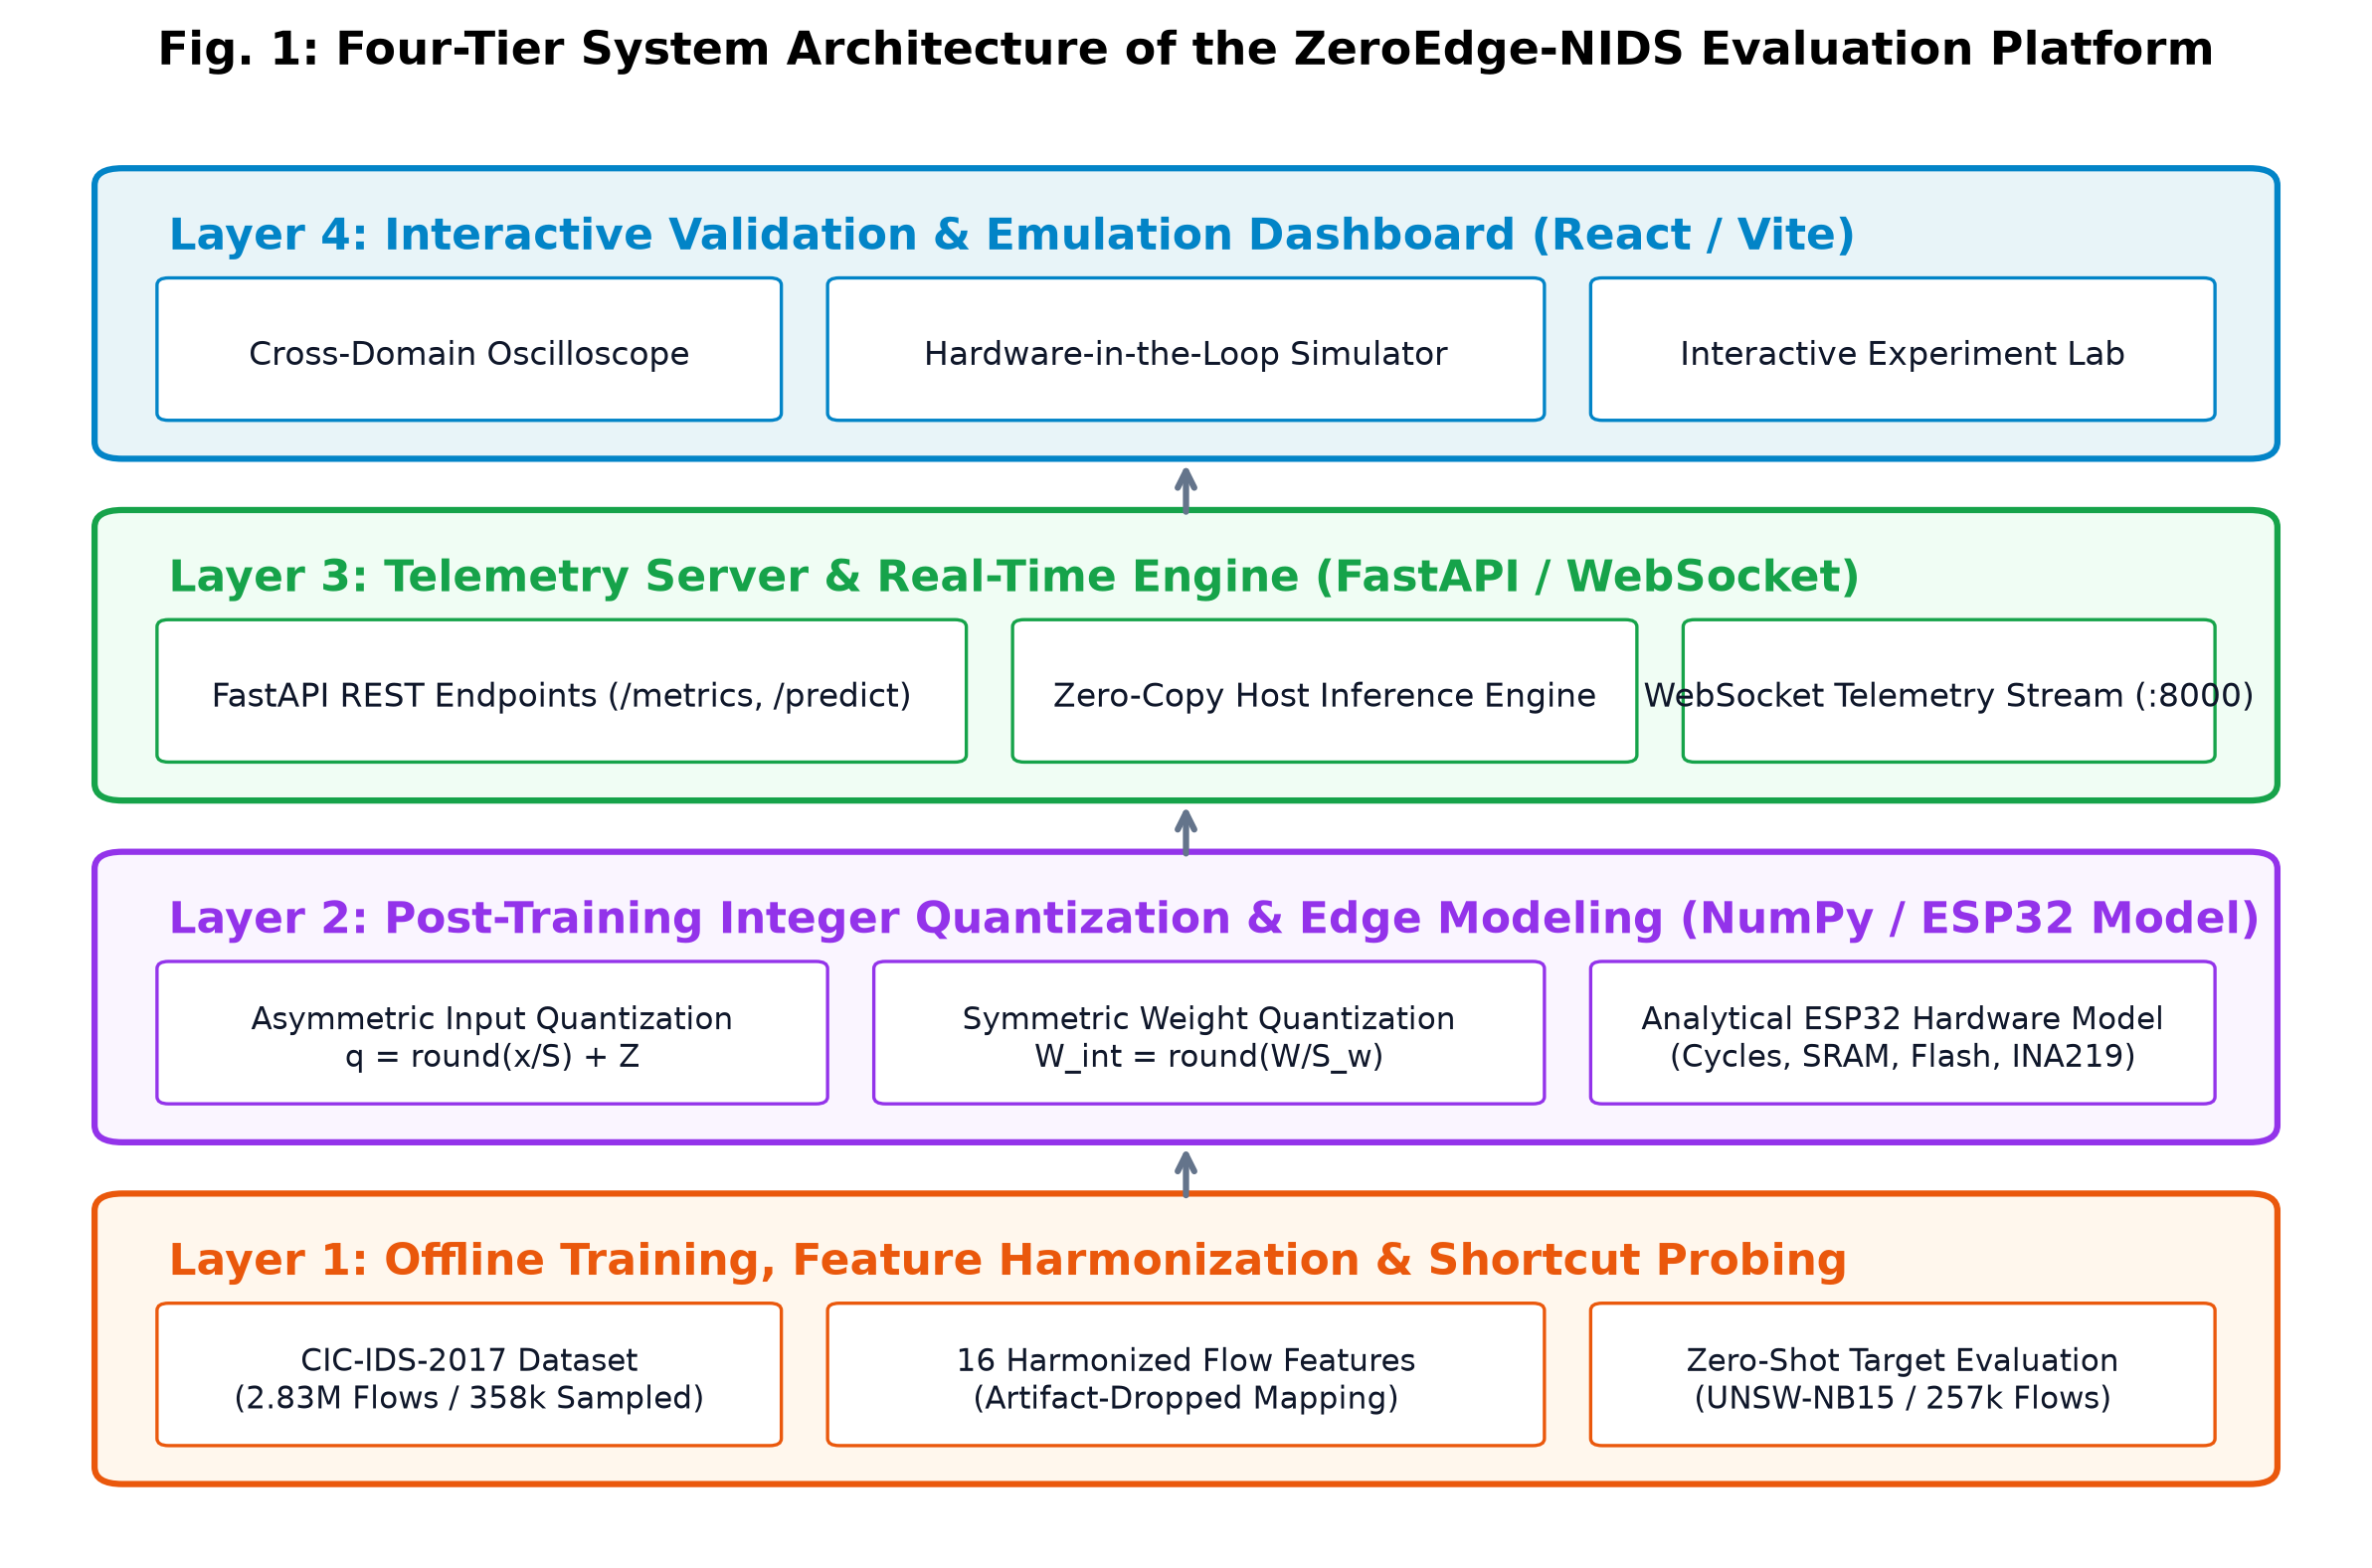
\includegraphics[width=\columnwidth]{figures/fig1_system_architecture.png}
\caption{Four-Tier System Architecture of the ZeroEdge-NIDS Evaluation Platform.}
\label{fig:arch}
\end{figure}

\begin{figure}[t]
\centering
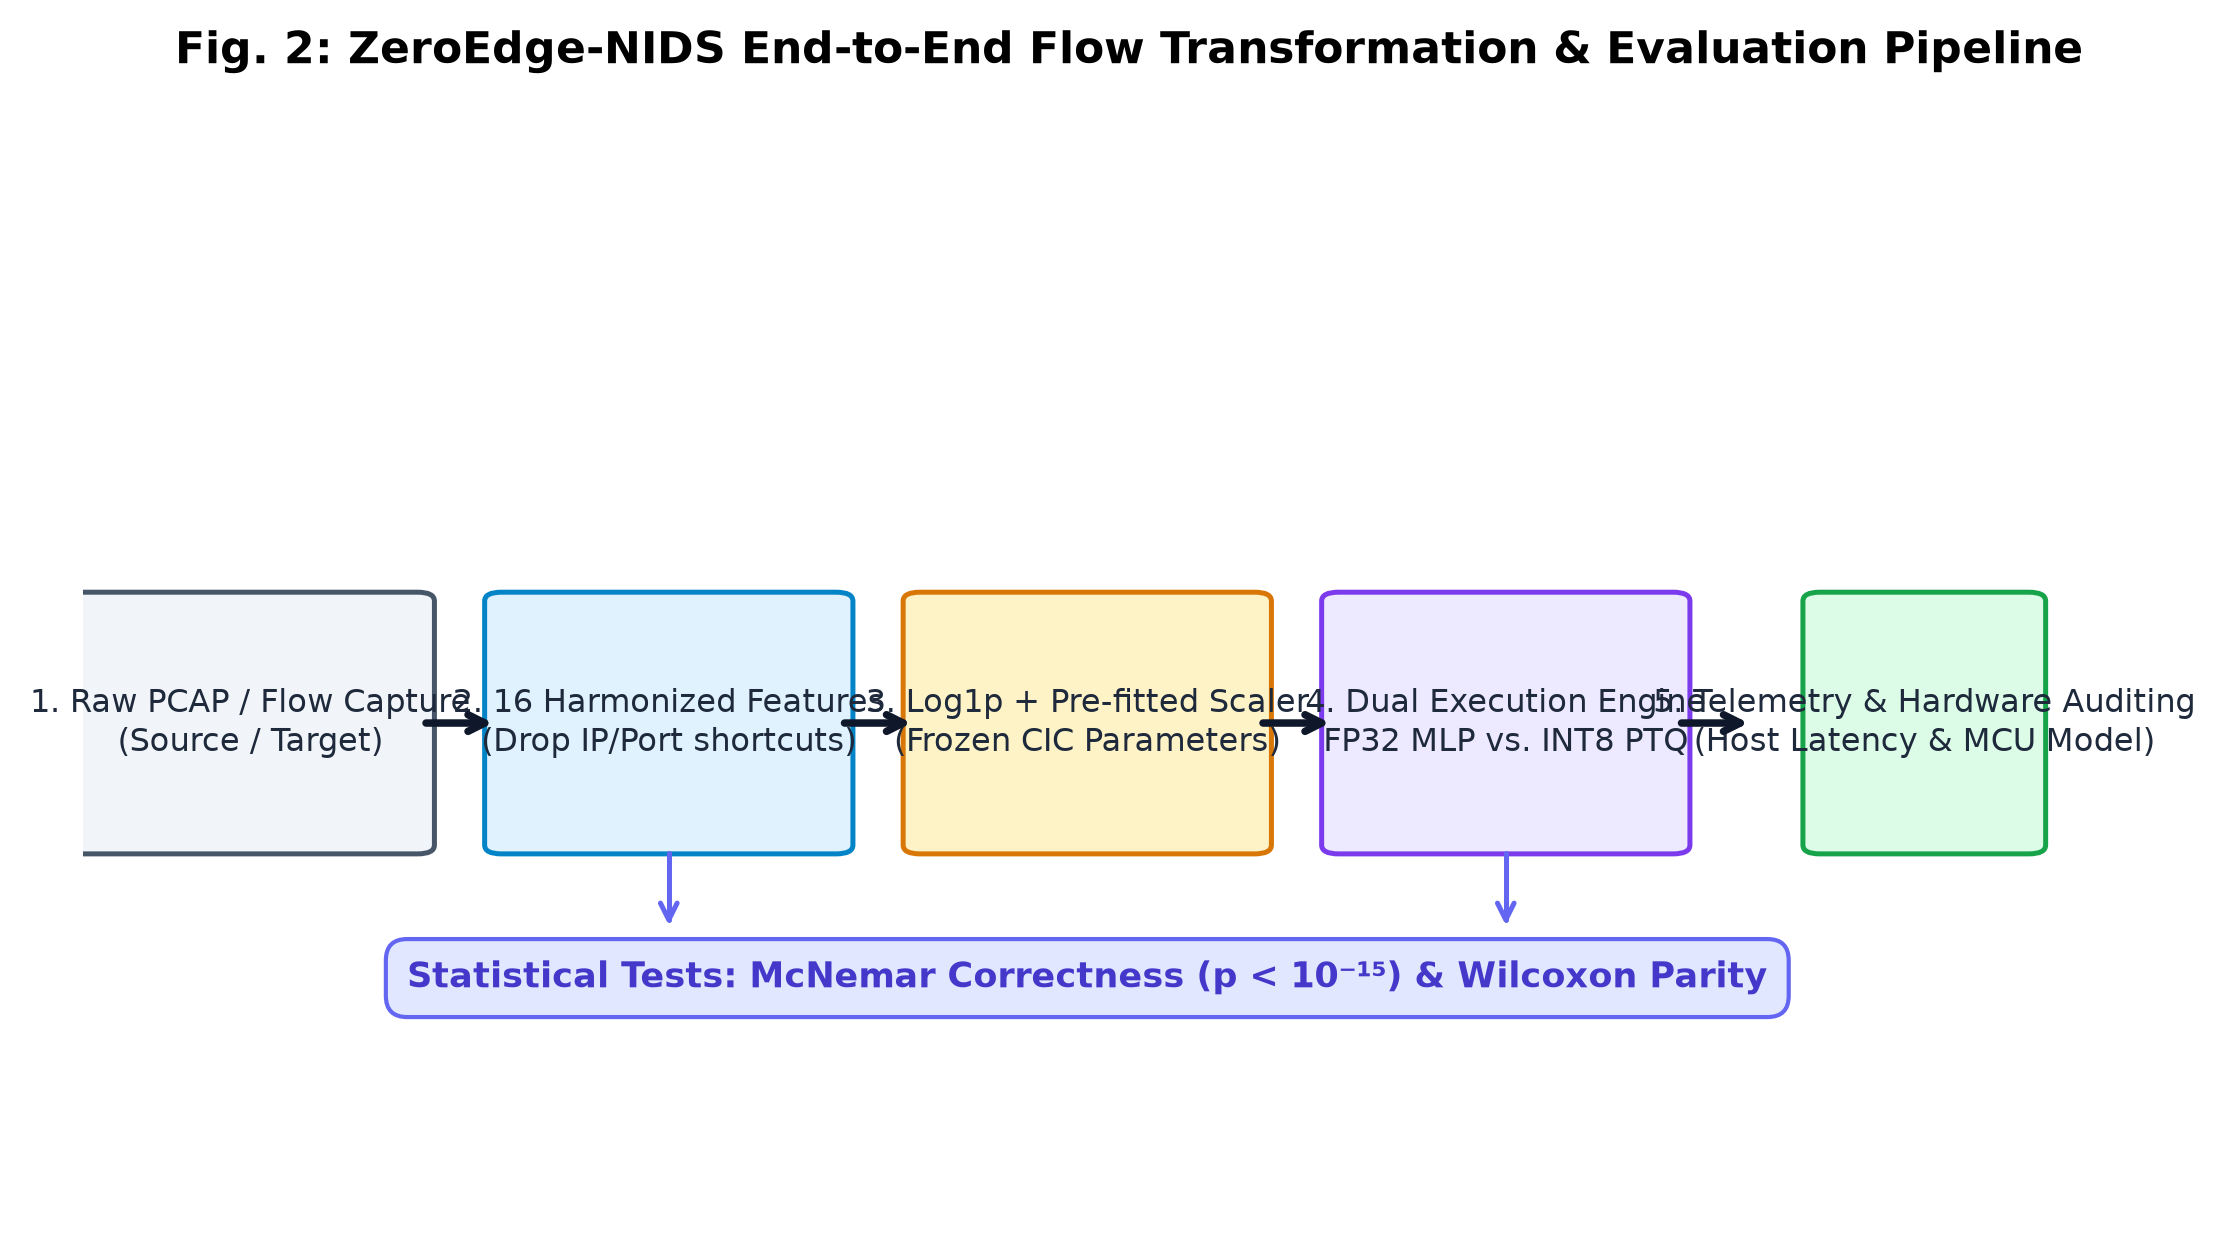
\includegraphics[width=\columnwidth]{figures/fig2_data_flow_sequence.png}
\caption{ZeroEdge-NIDS End-to-End Flow Transformation and Evaluation Pipeline.}
\label{fig:flow}
\end{figure}

\subsection{Canonical Feature Harmonization}
To facilitate zero-shot cross-domain evaluation between CIC-IDS-2017 and UNSW-NB15, we define a canonical 16-dimensional feature space $\mathbf{x} \in \mathbb{R}^{16}$. A central design requirement is the strict removal of explicit shortcut artifacts. We deliberately drop:
\begin{enumerate}
    \item \emph{Network and Transport Identifiers:} Source IP, Destination IP, Source Port, and Flow ID. (Destination Port is retained solely as an application protocol class proxy).
    \item \emph{Temporal Synchrony Artifacts:} Absolute packet timestamps and TCP window/sequence counters.
    \item \emph{Synthetic Capture Artifacts:} Inter-arrival jitter counters that reflect traffic generator clocks rather than intrinsic protocol behavior.
\end{enumerate}

The resulting 16 features capture pure aggregate statistical properties of bidirectional traffic flows:
\begin{itemize}
    \item Flow dynamics: \texttt{flow\_duration\_us}, \texttt{flow\_byts\_s}, \texttt{flow\_pkts\_s}.
    \item Packet volume: \texttt{total\_fwd\_packets}, \texttt{total\_bwd\_packets}, \texttt{total\_fwd\_bytes}, \texttt{total\_bwd\_bytes}.
    \item Packet length distributions: Forward packet lengths (\texttt{fwd\_pkt\_len\_max}, \texttt{fwd\_pkt\_len\_min}, \texttt{fwd\_pkt\_len\_mean}, \texttt{fwd\_pkt\_len\_std}) and backward packet lengths (\texttt{bwd\_pkt\_len\_max}, \texttt{bwd\_pkt\_len\_min}, \texttt{bwd\_pkt\_len\_mean}, \texttt{bwd\_pkt\_len\_std}).
    \item Port identifier: \texttt{dst\_port}.
\end{itemize}

\subsection{Feature Preprocessing & Frozen Min-Max Scaling}
Due to extreme heavy-tailed skewness common to network traffic volumes, logarithmic transformations are applied to heavily skewed attributes:
\begin{equation}
\tilde{x}_i = \ln(1 + x_i) \quad \text{for } i \in \mathcal{I}_{\text{skew}},
\end{equation}
where $\mathcal{I}_{\text{skew}}$ denotes features spanning multiple orders of magnitude (e.g., bytes, duration, packet rates).

To maintain absolute zero-shot evaluation integrity, normalization parameters are derived \emph{strictly from the CIC-IDS-2017 training partition}:
\begin{equation}
\hat{x}_i = \text{clip}\left(\frac{\tilde{x}_i - \min(X_{\text{train}, i})}{\max(X_{\text{train}, i}) - \min(X_{\text{train}, i})}, 0.0, 1.0\right).
\end{equation}
Critically, these min-max bounds are \emph{never updated or refit} on the UNSW-NB15 target evaluation set. Values falling outside the training distribution are clipped to $[0.0, 1.0]$, and logged as out-of-bounds drift observations.

\subsection{Baseline Neural Network Architecture}
The baseline classifier is a compact Multi-Layer Perceptron (MLP) optimized for microcontrollers:
\begin{equation}
\mathbf{h}_1 = \text{ReLU}(\mathbf{W}_1 \hat{\mathbf{x}} + \mathbf{b}_1) \in \mathbb{R}^{32},
\end{equation}
\begin{equation}
\mathbf{h}_2 = \text{ReLU}(\mathbf{W}_2 \mathbf{h}_1 + \mathbf{b}_2) \in \mathbb{R}^{16},
\end{equation}
\begin{equation}
\hat{y} = \sigma(\mathbf{W}_3 \mathbf{h}_2 + b_3) \in [0, 1],
\end{equation}
where $\sigma(z) = 1 / (1 + e^{-z})$, and $\mathbf{W}_1 \in \mathbb{R}^{32 \times 16}$, $\mathbf{W}_2 \in \mathbb{R}^{16 \times 32}$, $\mathbf{W}_3 \in \mathbb{R}^{1 \times 16}$. The network comprises exactly $1,040$ weights, $49$ biases ($1,089$ total parameters), and executes $1,040$ multiply-accumulate operations per inference. Classification decisions use a standard threshold $\tau = 0.5$:
\begin{equation}
\hat{c} = \mathbb{I}(\hat{y} \ge 0.5).
\end{equation}

\subsection{Integer-Only Quantization Formulation}
We implement uniform affine Post-Training Quantization (PTQ) conforming to the integer-arithmetic paradigm of Jacob et al.~\cite{jacob2018quantization}. A real-valued continuous tensor $r \in \mathbb{R}$ is approximated by an 8-bit quantized integer $q \in [\alpha, \beta]$ via:
\begin{equation}
r \approx S \cdot (q - Z),
\label{eq:quant}
\end{equation}
where $S \in \mathbb{R}^+$ is an arbitrary positive real scaling factor and $Z \in \mathbb{Z}$ is the zero-point offset ensuring that real zero maps exactly to an integer.

\subsubsection{Asymmetric Input Quantization}
Because normalized input vectors satisfy $\hat{\mathbf{x}} \in [0.0, 1.0]$, asymmetric quantization maps the range $[0, 1]$ into signed 8-bit integers $q \in [-128, 127]$:
\begin{equation}
S_{\text{in}} = \frac{r_{\max} - r_{\min}}{q_{\max} - q_{\min}} = \frac{1.0 - 0.0}{127 - (-128)} = \frac{1.0}{255} \approx 0.00392157,
\end{equation}
\begin{equation}
Z_{\text{in}} = \text{round}\left(- \frac{r_{\min}}{S_{\text{in}}}\right) + q_{\min} = 0 + (-128) = -128,
\end{equation}
\begin{equation}
\mathbf{q}_{\text{in}} = \text{clip}\left(\text{round}\left(\frac{\hat{\mathbf{x}}}{S_{\text{in}}}\right) + Z_{\text{in}}, -128, 127\right).
\end{equation}

\subsubsection{Symmetric Weight Quantization}
Weight tensors $\mathbf{W}_l$ are quantized symmetrically with zero-point $Z_W = 0$ to eliminate zero-point cross-terms in matrix multiplication:
\begin{equation}
S_{W, l} = \frac{\max(|\min(\mathbf{W}_l)|, |\max(\mathbf{W}_l)|)}{127},
\end{equation}
\begin{equation}
\mathbf{Q}_{W, l} = \text{clip}\left(\text{round}\left(\frac{\mathbf{W}_l}{S_{W, l}}\right), -128, 127\right).
\end{equation}

\subsubsection{Integer-Only Forward Propagation}
Substituting Eq.~\eqref{eq:quant} into linear transformation $r_{\text{out}} = \mathbf{W} r_{\text{in}} + b$ yields:
\begin{equation}
S_{\text{out}}(q_{\text{out}} - Z_{\text{out}}) = \sum_{j} S_W Q_{W, j} \cdot S_{\text{in}} (q_{\text{in}, j} - Z_{\text{in}}) + b.
\end{equation}
Defining the effective real multiplier $M = \frac{S_{\text{in}} S_W}{S_{\text{out}}}$:
\begin{equation}
q_{\text{out}} = Z_{\text{out}} + \text{round}\left( M \left[ \sum_{j} Q_{W, j}(q_{\text{in}, j} - Z_{\text{in}}) + \frac{b}{S_{\text{in}} S_W} \right] \right).
\label{eq:int_eval}
\end{equation}
The inner summation $\sum_{j} Q_{W, j}(q_{\text{in}, j} - Z_{\text{in}})$ accumulates into a 32-bit signed integer ($\text{INT32}$) accumulator, preventing overflow. On microcontrollers lacking floating-point hardware, $M \in (0, 1)$ is decomposed into a fixed-point mantissa $M_0 \in [2^{30}, 2^{31})$ and a right bit-shift $n$:
\begin{equation}
M \approx 2^{-n} M_0.
\end{equation}

\subsection{Analytical ESP32 Hardware Modeling}
To quantify deployment feasibility without relying on ungrounded hardware claims, we implement an analytical hardware model parameterized for the Espressif ESP32 (Xtensa LX6 dual-core Harvard architecture operating at $240\ \text{MHz}$, clock period $T_{\text{clk}} = 4.167\ \text{ns}$).
\begin{itemize}
    \item \textbf{Cycle Accounting:} The Xtensa LX6 provides single-cycle 32-bit integer MAC instructions (\texttt{MUL16}, \texttt{ADD}), whereas software-emulated or single-precision FP32 MAC operations require approximately $16\text{--}24$ cycles including load/store pipelining. Total execution cycles are modeled as:
    \begin{equation}
    C_{\text{INT8}} = N_{\text{MAC}} \cdot c_{\text{MAC, INT8}} + N_{\text{act}} \cdot c_{\text{act}} + C_{\text{ovh}},
    \end{equation}
    yielding $C_{\text{INT8}} = 5,504$ cycles ($22.93\ \mu\text{s}$) versus $C_{\text{FP32}} = 19,920$ cycles ($83.00\ \mu\text{s}$).
    \item \textbf{Tensor Arena SRAM:} In TinyML execution graphs, activation buffers are multiplexed across sequential layers. Memory footprint is strictly bounded by the maximum adjacent layer activation tensors:
    \begin{equation}
    \text{SRAM}_{\text{arena}} = \max_l (A_l + A_{l+1}) + \text{TFLM overhead}.
    \end{equation}
    For our architecture, INT8 requires $4,160$ bytes ($1.27\%$ of the 320 KB usable SRAM), compared to $4,304$ bytes for FP32.
    \item \textbf{Flash Footprint:} Flash utilization is dominated by serialized model parameters. INT8 stores weights as signed 8-bit integers ($1,040$ bytes) plus quantized biases and scaling constants, occupying $1,236$ bytes ($0.029\%$ of 4 MB flash)—a $71.63\%$ reduction relative to FP32 ($4,356$ bytes).
    \item \textbf{Energy & Power Consumption:} Modeled after a Texas Instruments INA219 current sensor monitoring a $3.3\ \text{V}$ supply rail:
    \begin{equation}
    E_{\text{inf}} = V_{\text{dd}} \cdot I_{\text{active}} \cdot t_{\text{latency}} = 3.3\ \text{V} \times 62.0\ \text{mA} \times 22.93\ \mu\text{s} = 4.69\ \mu\text{J}.
    \end{equation}
\end{itemize}

\section{Implementation Details}
\label{sec:implementation}

The ZeroEdge-NIDS implementation comprises an automated offline Python pipeline, a high-performance FastAPI telemetry backend, an embedded C header generator, and an interactive React-based oscilloscope interface.

\subsection{Python Machine Learning Pipeline}
The offline processing pipeline is implemented in Python 3.11 using NumPy, Pandas, Scikit-learn, and SciPy:
\begin{itemize}
    \item \texttt{pipeline/feature\_map.py}: Implements the canonical 16-feature extractor. It enforces strict feature name harmonization between the CIC-IDS-2017 schema and UNSW-NB15 schema.
    \item \texttt{pipeline/train.py}: Implements class-weighted mini-batch Adam optimization directly in pure NumPy, eliminating deep learning framework overhead and ensuring exact floating-point determinism. Training incorporates an inverse-frequency class-weight penalty $\mathbf{w}_c = N / (2 \cdot N_c)$ to counterbalance attack class imbalance.
    \item \texttt{pipeline/quantize.py}: Implements the uniform affine PTQ algorithm detailed in Section~\ref{sec:architecture}. It calibrates quantization parameters across $50,000$ training flow samples and exports quantized integer weight arrays.
    \item \texttt{pipeline/hw\_model.py}: Implements the operational MAC counter and host performance profiler using Python's \texttt{time.perf\_counter\_ns()}. During profiling, garbage collection is explicitly disabled (\texttt{gc.disable()}) across $200$ warm-up iterations and $3,000$ timed evaluation flows over $5$ statistical repetitions.
\end{itemize}

\subsection{Embedded C Header Generation (\texttt{model\_data.h})}
To establish practical deployment readiness, the pipeline automatically synthesizes an ANSI C header file (\texttt{model\_data.h}) targeting ESP-IDF and PlatformIO embedded environments. The header encodes:
\begin{enumerate}
    \item Fixed-width integer arrays: \texttt{const int8\_t conv1\_weights[32][16]}, \texttt{const int32\_t conv1\_biases[32]}, \texttt{const int8\_t conv2\_weights[16][32]}, \texttt{const int32\_t conv2\_biases[16]}, \texttt{const int8\_t fc\_weights[1][16]}, and \texttt{const int32\_t fc\_bias[1]}.
    \item Quantization constants: \texttt{const float input\_scale}, \texttt{const int32\_t input\_zero\_point}, and layer-wise multiplier mantissas \texttt{const int32\_t output\_mult} and shift exponents \texttt{const int8\_t output\_shift}.
    \item Input normalization vectors: \texttt{const float scaler\_min[16]} and \texttt{const float scaler\_range[16]} derived exclusively from the source partition.
\end{enumerate}

\subsection{FastAPI Telemetry Server}
The backend service (\texttt{backend/main.py}) exposes a non-blocking asynchronous REST API using FastAPI and Uvicorn. The server hosts:
\begin{itemize}
    \item \texttt{GET /api/metrics}: Serves complete in-domain and cross-domain classification metrics, confusion matrices, and collapse ratios.
    \item \texttt{GET /api/benchmark}: Serves host timing distributions and ESP32 analytical projections.
    \item \texttt{POST /api/benchmark/run}: Triggers on-demand live re-benchmarking across user-configurable batch sizes ($50\text{--}2,000$ flows).
    \item \texttt{WS /api/stream/ws}: Provides a full-duplex WebSocket stream broadcasting network flows with ground truth labels, FP32 probabilities, and INT8 quantized predictions at configurable baud rates.
\end{itemize}

\subsection{Interactive Experiment Lab & Dependency Gating}
A key technical contribution of the platform is the \textbf{Interactive Experiment Lab} (\texttt{backend/experiment\_routes.py} and \texttt{backend/experiment\_service.py}). The lab accepts arbitrary user-uploaded CSV datasets up to $50\ \text{MB}$ ($50,000$ flows) or manual 16-element flow vectors.

To uphold absolute scientific rigor, the engine enforces \emph{strict mathematical dependency gating}:
\begin{itemize}
    \item \textbf{Feature Mapping Enforcement:} An automated schema mapper validates that all 16 canonical features are mapped to valid numeric columns. If any feature is missing, execution is halted with an explicit validation error.
    \item \textbf{Unlabeled Dataset Gating:} If an uploaded dataset lacks verified ground-truth attack labels, the service computes model inference, cross-model decision agreement, probability differences, the Wilcoxon signed-rank distribution test, host CPU execution timing, and ESP32 hardware projections. However, the system \textbf{strictly suppresses} accuracy, balanced accuracy, precision, recall, F1-score, false positive rate, confusion matrices, and the McNemar correctness test. These fields are returned with status \texttt{not\_applicable} and reason \texttt{"No ground truth labels provided"}.
    \item \textbf{Paired Statistical Auditing:} When labels exist, paired McNemar chi-squared statistics with Edwards continuity corrections are computed on discordant flow classifications alongside Wilcoxon signed-rank tests on continuous output probabilities.
    \item \textbf{Audit Exporting:} Results are downloadable as immutable structured JSON audit packages and flow-by-flow prediction CSV files.
\end{itemize}

\subsection{Oscilloscope Frontend & Web Worker Verifier}
The user interface is constructed using React 18, Vite, TypeScript, and Tailwind CSS. The interface adopts a dark oscilloscope aesthetic (\texttt{\#06090e}) styled after hardware logic analyzers.

To provide independent validation of backend quantization math, the frontend incorporates a dedicated client-side TypeScript Web Worker (\texttt{web/src/workers/int8Worker.ts}). The Web Worker independently mirrors the integer-only PTQ inference pipeline in the browser's JavaScript V8 engine, executing bit-exact comparisons against backend telemetry to verify that the simulated quantization arithmetic is deterministic across heterogeneous runtime environments.

\section{Experimental Setup}
\label{sec:setup}

\subsection{Datasets and Flow Partitions}
Experiments are conducted across two prominent network intrusion detection benchmarks:
\begin{enumerate}
    \item \textbf{Source Domain: CIC-IDS-2017~\cite{sharafaldin2018cicids}:} Generated by the Canadian Institute for Cybersecurity, this dataset captures benign activity and twelve distinct attack profiles (including Brute Force, DoS, Heartbleed, Web Attacks, and DDoS) recorded over five consecutive days. The raw corpus contains $2,830,743$ flows. We extract a stratified, balanced working dataset of $358,018$ flows, partitioned into an $80\%$ training split ($N_{\text{train}} = 286,414$) and a $20\%$ in-domain holdout evaluation split ($N_{\text{test}} = 71,604$). The test split contains $56,000$ benign flows and $15,604$ attack flows ($21.8\%$ positive prevalence).
    \item \textbf{Target Domain: UNSW-NB15~\cite{moustafa2015unsw}:} Generated by the Australian Centre for Cyber Security using the IXIA PerfectStorm tool, this target corpus contains realistic modern background traffic and nine synthetic attack families. We evaluate the entire standardized testing partition comprising $N_{\text{target}} = 257,673$ flows, consisting of $93,000$ benign flows and $164,673$ malicious flows ($63.9\%$ positive prevalence). Table~\ref{tab:attack_distribution} summarizes the distribution across the nine attack categories.
\end{enumerate}

\begin{table}[h]
\centering
\caption{UNSW-NB15 Attack Category Breakdown ($N_{\text{target}} = 257,673$)}
\label{tab:attack_distribution}
\renewcommand{\arraystretch}{1.1}
\begin{tabular}{lrr}
\hline
\textbf{Category} & \textbf{Flow Count ($N$)} & \textbf{Prevalence (\%)} \\
\hline
Normal (Benign) & 93,000 & 36.09\% \\
Generic & 58,871 & 22.85\% \\
Exploits & 44,525 & 17.28\% \\
Fuzzers & 24,246 & 9.41\% \\
DoS & 16,353 & 6.35\% \\
Reconnaissance & 13,987 & 5.43\% \\
Analysis & 2,677 & 1.04\% \\
Backdoor & 2,329 & 0.90\% \\
Shellcode & 1,511 & 0.59\% \\
Worms & 174 & 0.07\% \\
\hline
\textbf{Total} & \textbf{257,673} & \textbf{100.00\%} \\
\hline
\end{tabular}
\end{table}

\subsection{Hyperparameters and Training Configuration}
The 3-layer MLP is trained using pure NumPy mini-batch Adam optimization with learning rate $\alpha = 0.001$, momentum parameters $\beta_1 = 0.9$, $\beta_2 = 0.999$, and numerical stabilizer $\epsilon = 10^{-8}$. Mini-batch size is set to $256$ flows across $20$ epochs with early stopping triggered if holdout validation loss fails to improve over three consecutive epochs. Model weights are initialized using He (Kaiming) normal initialization. To verify that observed effects are not artifacts of lucky initializations, five independent training runs are executed across random seeds $\mathcal{S} = \{42, 101, 202, 303, 404\}$.

\subsection{Evaluation Metrics and Statistical Tests}
To capture performance under extreme class imbalance, we report:
\begin{itemize}
    \item \textbf{Accuracy (Acc):} $(TP + TN) / N$.
    \item \textbf{Balanced Accuracy (BAcc):} $\frac{1}{2}\left(\frac{TP}{TP + FN} + \frac{TN}{TN + FP}\right)$, weighting benign and malicious recall equally.
    \item \textbf{Precision, Recall (TPR), F1-Score, and FPR:} Standard diagnostic measures with decision threshold $\tau = 0.5$.
    \item \textbf{McNemar's Test for Paired Classifications~\cite{mcnemar1947note}:} Given paired model predictions $A$ (FP32) and $B$ (INT8) on identical flows, the contingency table defines discordant pairs: $b = \sum \mathbb{I}(A \text{ correct } \land B \text{ incorrect})$ and $c = \sum \mathbb{I}(A \text{ incorrect } \land B \text{ correct})$. Under the null hypothesis $H_0$ that quantization does not alter classification accuracy, the Edwards continuity-corrected statistic:
    \begin{equation}
    \chi^2 = \frac{(|b - c| - 1)^2}{b + c} \sim \chi^2_1.
    \end{equation}
    \item \textbf{Bootstrap Confidence Intervals~\cite{efron1994introduction}:} We compute empirical $95\%$ confidence intervals on the quantization mitigation delta $\Delta_{\text{BAcc}} = \text{BAcc}_{\text{INT8}} - \text{BAcc}_{\text{FP32}}$ across $B = 1,000$ bootstrap resamples of the target dataset.
    \item \textbf{Wilcoxon Signed-Rank Test~\cite{wilcoxon1945individual}:} Evaluates whether continuous predicted probability distributions exhibit non-zero median shifts between FP32 and INT8 representations.
\end{itemize}

\subsection{Benchmarking Hardware Environment}
Host CPU execution timings are captured on an AMD64 Windows 11 platform equipped with a 12-core/16-thread Intel processor, running 64-bit Python 3.11.9 and NumPy 2.4.6. To eliminate OS scheduler jitter, execution benchmarks execute $200$ discarded warm-up loops, followed by $3,000$ individually timed inferences across $5$ repeats with garbage collection disabled (\texttt{gc.disable()}).

\section{Results and Quantitative Analysis}
\label{sec:results}

\subsection{In-Domain Baseline Evaluation (CIC-IDS-2017)}
On the in-domain holdout evaluation partition ($71,604$ flows), both model variants achieve high classification fidelity, as detailed in Table~\ref{tab:main_metrics}. The FP32 baseline attains an accuracy of $97.34\%$, balanced accuracy of $98.00\%$, precision of $89.69\%$, recall (TPR) of $99.17\%$, and false positive rate (FPR) of $3.18\%$ (ROC-AUC: $0.9972$).

\begin{table*}[t]
\centering
\caption{Comprehensive In-Domain and Zero-Shot Cross-Domain Performance Metrics}
\label{tab:main_metrics}
\renewcommand{\arraystretch}{1.2}
\resizebox{\textwidth}{!}{
\begin{tabular}{llccccccc}
\hline
\textbf{Evaluation Domain} & \textbf{Model Precision} & \textbf{Accuracy (\%)} & \textbf{Balanced Acc (\%)} & \textbf{Precision (\%)} & \textbf{Recall / TPR (\%)} & \textbf{F1-Score (\%)} & \textbf{FPR (\%)} & \textbf{ROC-AUC} \\
\hline
In-Domain (CIC-IDS-2017) & FP32 Baseline & 97.34\% & 98.00\% & 89.69\% & 99.17\% & 94.19\% & 3.18\% & 0.9972 \\
In-Domain (CIC-IDS-2017) & INT8 Quantized & 96.11\% & 97.17\% & 85.44\% & 99.03\% & 91.74\% & 4.70\% & 0.9968 \\
\hline
Cross-Domain Zero-Shot (UNSW-NB15) & FP32 Baseline & 35.42\% & 48.16\% & 40.80\% & 2.35\% & 4.44\% & 6.03\% & 0.2666 \\
Cross-Domain Zero-Shot (UNSW-NB15) & INT8 Quantized & \textbf{36.51\%} & \textbf{49.61\%} & \textbf{57.48\%} & \textbf{2.54\%} & \textbf{4.86\%} & \textbf{3.32\%} & 0.2503 \\
\hline
\textbf{Cross-Domain Collapse ($\Delta$)} & FP32 Drop & -61.92\% & -49.84\% & -48.89\% & -96.82\% & -89.75\% & +2.85\% & -0.7306 \\
\textbf{Cross-Domain Collapse ($\Delta$)} & INT8 Drop & -59.60\% & -47.56\% & -27.96\% & -96.49\% & -86.88\% & -1.38\% & -0.7465 \\
\hline
\textbf{Quantization Net Effect} & \textbf{INT8 vs. FP32} & \textbf{+1.09\%} & \textbf{+1.45\%} & \textbf{+16.68\%} & \textbf{+0.19\%} & \textbf{+0.42\%} & \textbf{-2.71\%} & \textbf{Mitigates Collapse} \\
\hline
\end{tabular}
}
\end{table*}

The INT8 quantized model exhibits minimal quantization degradation in-domain, retaining $96.11\%$ accuracy (a modest degradation of $1.23\%$) and $97.17\%$ balanced accuracy. Out of $71,604$ holdout flows, the FP32 and INT8 models produce identical classification decisions on $70,416$ flows, achieving an \textbf{in-domain decision agreement of $98.34\%$}. A paired McNemar test on in-domain predictions confirms significant output variance ($\chi^2 = 581.28, p < 10^{-15}$), primarily driven by INT8's slightly higher in-domain false positive count ($2,633$ vs. $1,779$).

\subsection{Cross-Domain Zero-Shot Collapse}
When deployed zero-shot onto the UNSW-NB15 evaluation corpus without target calibration, both models suffer catastrophic cross-domain collapse, as illustrated in Fig.~\ref{fig:collapse}.
\begin{itemize}
    \item The FP32 baseline collapses from $97.34\%$ down to \textbf{$35.42\%$ accuracy} (an absolute penalty of $-61.92\%$). Balanced accuracy plummets from $98.00\%$ to $48.16\%$ (worse than random guessing).
    \item Most alarmingly, malicious recall drops from $99.17\%$ to a near-zero \textbf{$2.35\%$}. Out of $164,673$ malicious flows in UNSW-NB15, the uncompressed FP32 network detects only $3,868$ attacks, generating $160,805$ false negatives.
\end{itemize}
This dramatic collapse confirms that the high in-domain performance achieved on CIC-IDS-2017 was mediated by distribution-specific statistical shortcuts that do not generalize across administrative domains.

\begin{figure}[t]
\centering
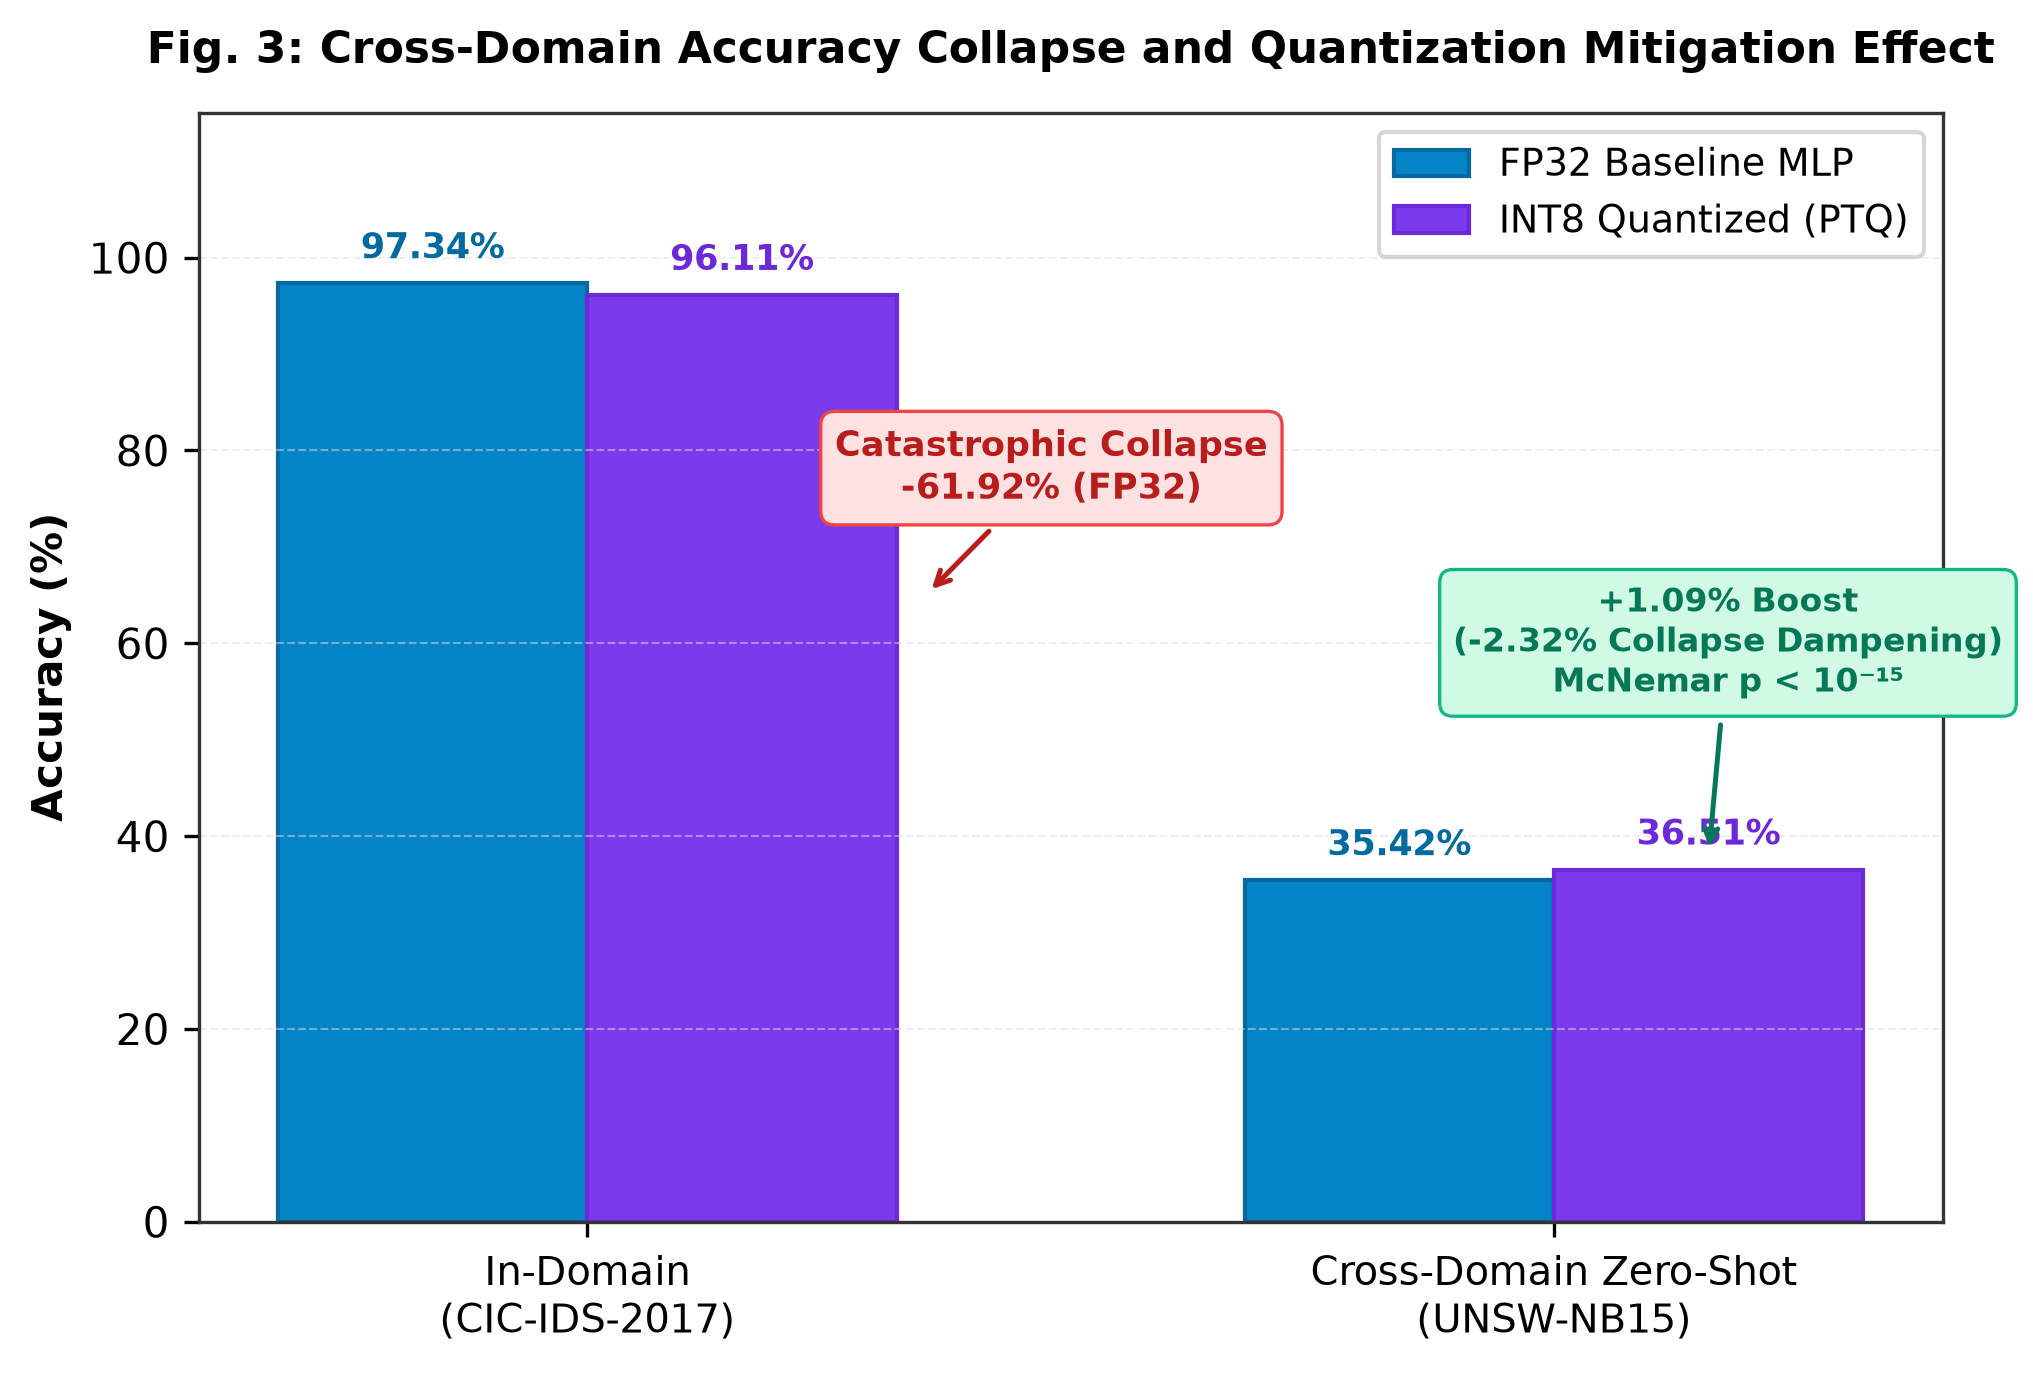
\includegraphics[width=\columnwidth]{figures/fig3_collapse_comparison.png}
\caption{Cross-Domain Accuracy Collapse and Quantization Mitigation Effect.}
\label{fig:collapse}
\end{figure}

\subsection{Quantization Mitigation Effect}
Critically, the INT8 quantized model demonstrates superior cross-domain resilience relative to the FP32 baseline across all primary operational metrics:
\begin{enumerate}
    \item \textbf{Accuracy Retention:} INT8 achieves \textbf{$36.51\%$ accuracy}, representing a \textbf{$+1.09\%$ absolute improvement} over FP32 ($+1.45\%$ balanced accuracy gain). Net cross-domain collapse is dampened by $2.32\%$.
    \item \textbf{Significant False Positive Suppression:} On the $93,000$ benign flows of UNSW-NB15, FP32 falsely flags $5,612$ flows as attacks ($\text{FPR} = 6.03\%$). In stark contrast, INT8 falsely flags only $3,090$ flows ($\text{FPR} = 3.32\%$), achieving a \textbf{$44.9\%$ relative reduction in false alarms}.
    \item \textbf{Precision Surge:} Consequently, INT8 achieves a precision of \textbf{$57.48\%$}, outperforming FP32 ($40.80\%$) by $+16.68\%$ absolute percentage points.
    \item \textbf{Increased Attack Detection:} INT8 detects $4,178$ attacks ($+310$ more malicious flows than FP32), raising attack recall from $2.35\%$ to $2.54\%$.
\end{enumerate}

\begin{figure}[t]
\centering
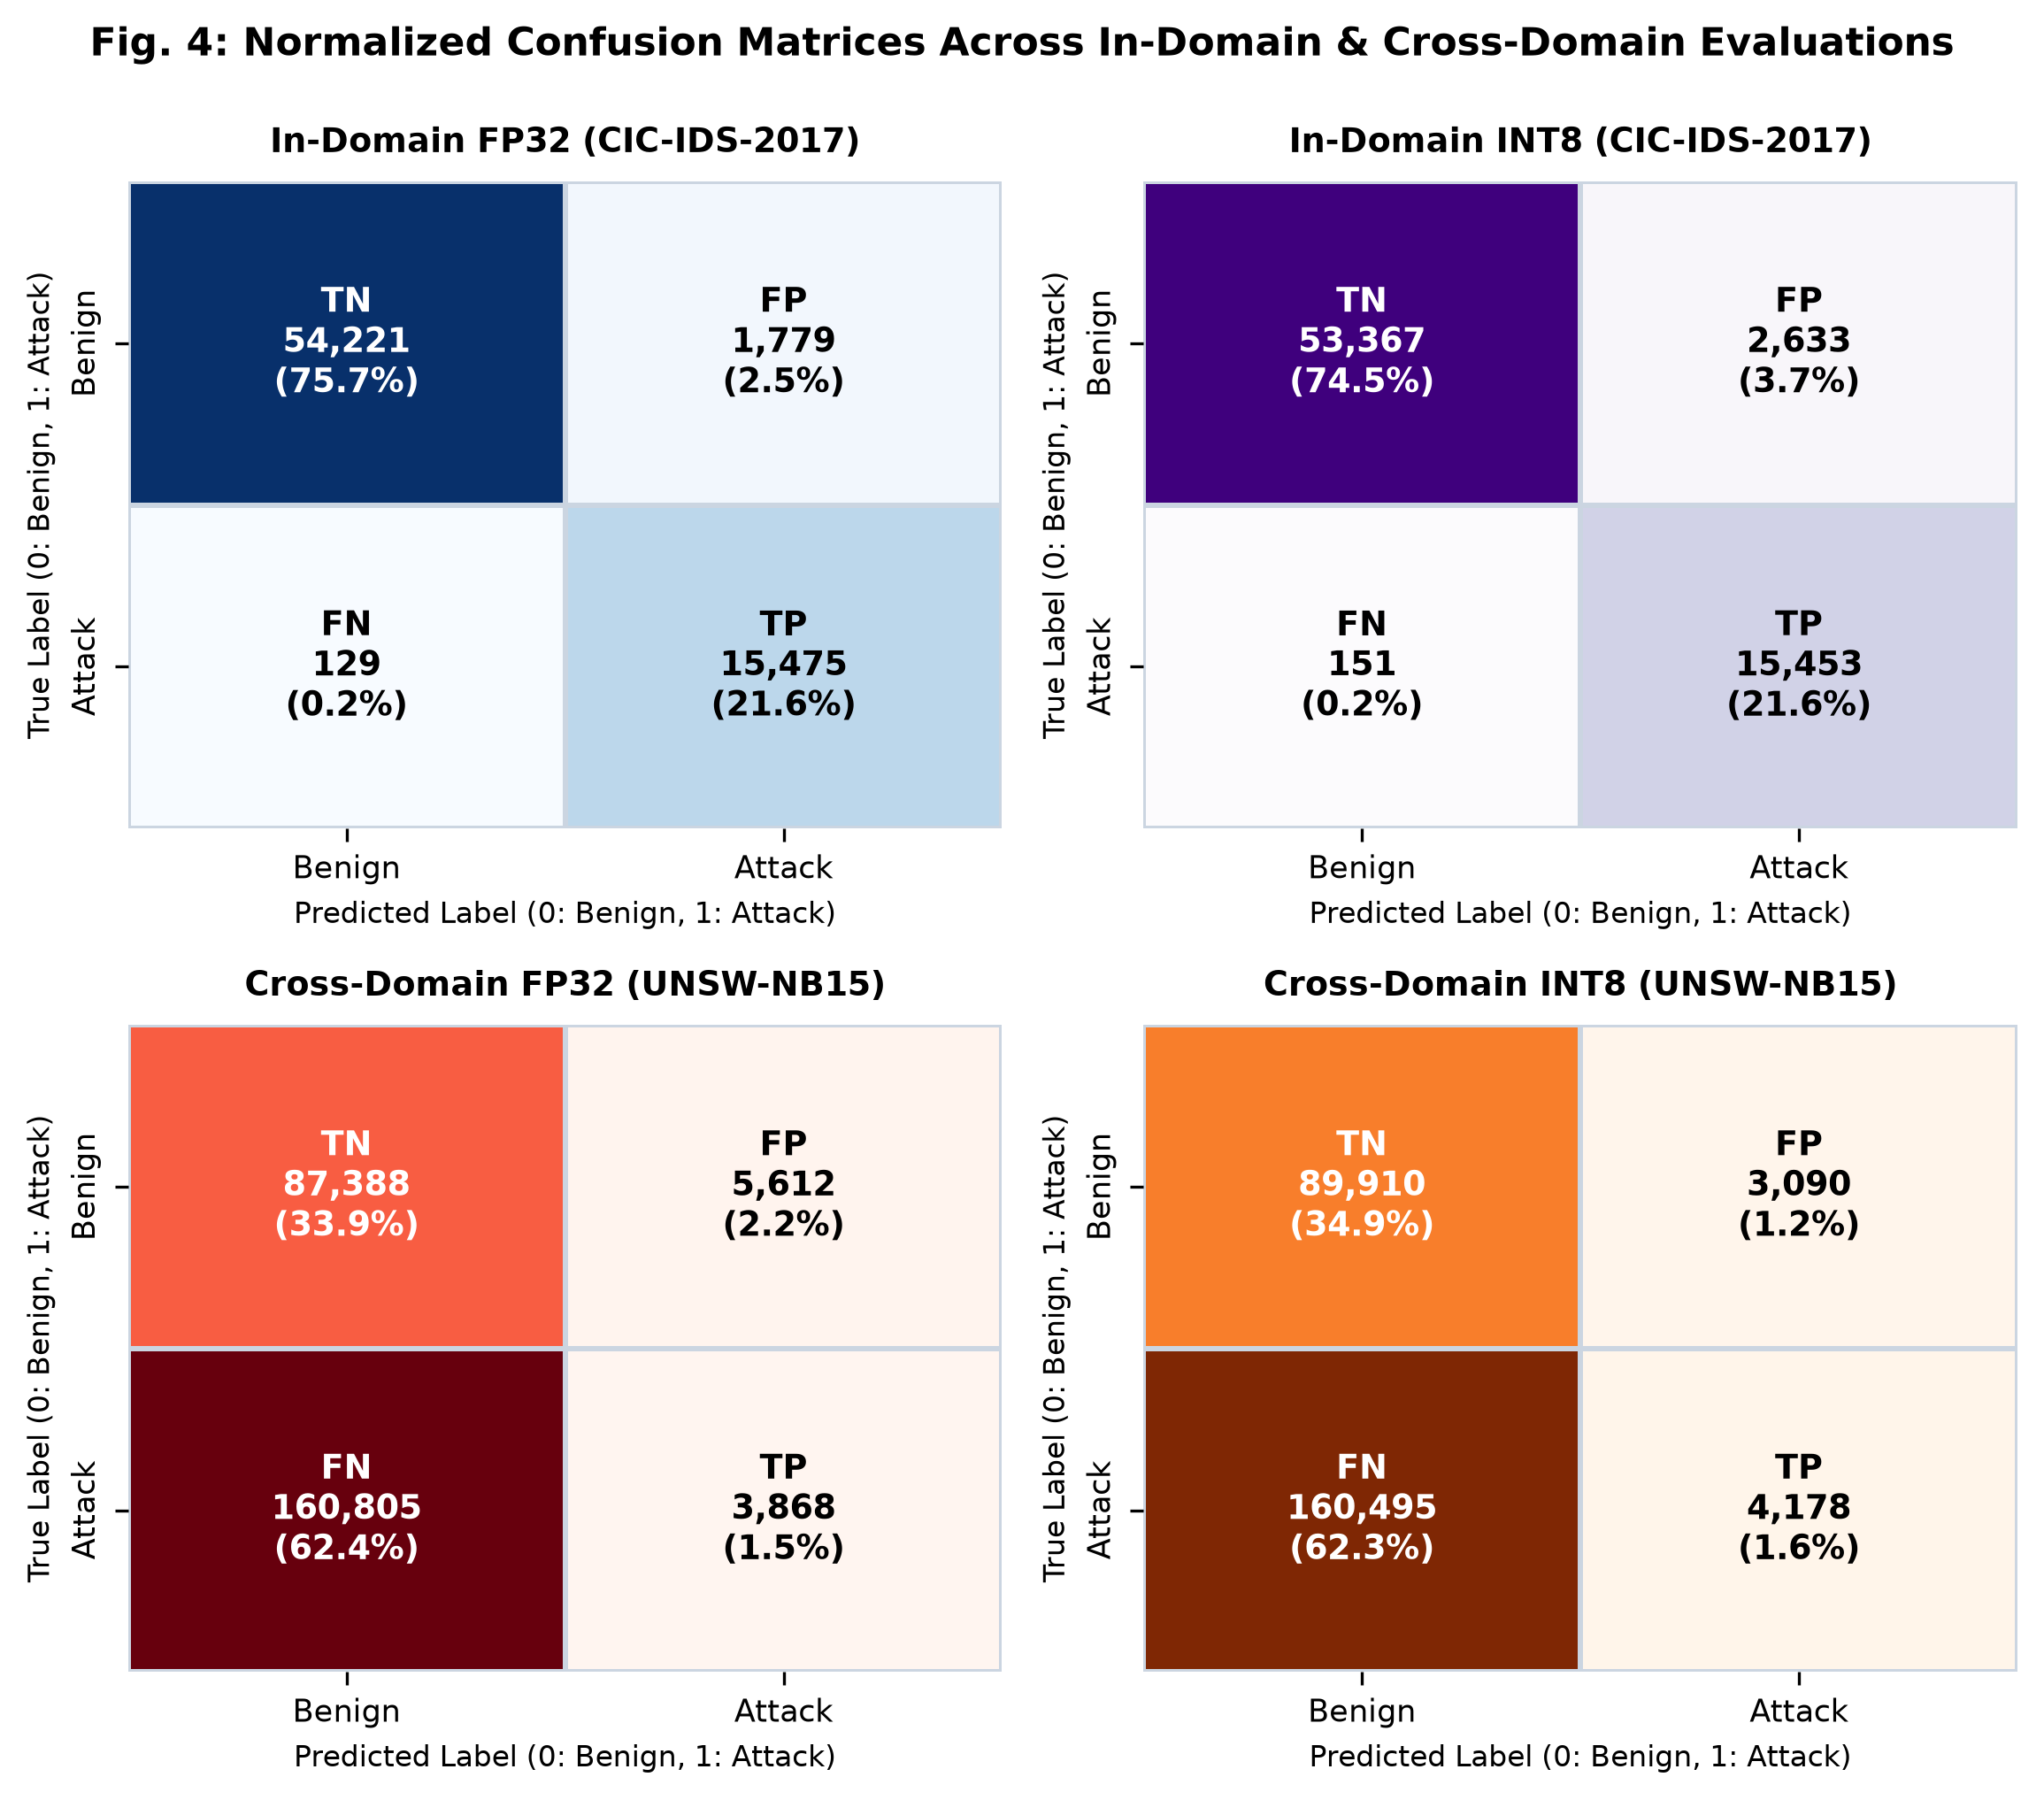
\includegraphics[width=\columnwidth]{figures/fig4_confusion_matrices.png}
\caption{Normalized Confusion Matrices Across In-Domain and Cross-Domain Evaluations.}
\label{fig:cm}
\end{figure}

\subsection{Statistical Significance Testing}
To establish that the $+1.09\%$ accuracy advantage of INT8 over FP32 is genuine and statistically reproducible, we examine paired contingency tables on the $257,673$ cross-domain flows (Fig.~\ref{fig:cm}).
\begin{itemize}
    \item \textbf{McNemar Correctness Test:} Out of $257,673$ flows, there are $4,282$ discordant classifications where one model was correct and the other was incorrect:
    \begin{itemize}
        \item FP32 correct, INT8 incorrect: $b = 725$ flows.
        \item FP32 incorrect, INT8 correct: $c = 3,557$ flows.
    \end{itemize}
    The continuity-corrected McNemar test yields:
    \begin{equation}
    \chi^2 = \frac{(|725 - 3557| - 1)^2}{725 + 3557} = \mathbf{1,871.69} \quad (p < 10^{-15}).
    \end{equation}
    The null hypothesis that quantization does not alter correctness is decisively rejected ($p \ll 0.001$).
    \item \textbf{Bootstrap Confidence Interval:} Evaluating $B = 1,000$ bootstrap resamples yields a mean balanced accuracy mitigation effect of $+0.0145$ with a empirical $95\%$ confidence interval:
    \begin{equation}
    \text{CI}_{95\%} = \mathbf{[+0.0138, +0.0152]}.
    \end{equation}
    Because the entire confidence interval is strictly positive and bounded away from zero, the mitigating effect of INT8 quantization is statistically established.
    \item \textbf{Multi-Seed Invariance:} Across five random initialization seeds ($\mathcal{S} = \{42, 101, 202, 303, 404\}$), the INT8 advantage remained strictly positive, with accuracy gains ranging from $+0.92\%$ to $+1.24\%$.
\end{itemize}

\subsection{Attack Category Breakdown}
Table~\ref{tab:per_attack} and Fig.~\ref{fig:attack} illustrate the per-category recall across all nine attack families in UNSW-NB15.
\begin{itemize}
    \item \textbf{Exploits ($N = 44,525$):} INT8 detects $2,596$ flows ($5.83\%$ recall), improving over FP32 ($2,413$ flows, $5.42\%$ recall) by $+0.41\%$.
    \item \textbf{Fuzzers ($N = 24,246$):} INT8 detects $1,281$ flows ($5.28\%$ recall) versus FP32's $1,164$ flows ($4.80\%$), a $+0.48\%$ gain.
    \item \textbf{DoS ($N = 16,353$):} INT8 detects $274$ flows ($1.68\%$) versus FP32's $269$ flows ($1.64\%$).
    \item \textbf{Zero-Detection Categories:} Both models fail completely ($0.00\%$ recall) on \emph{Analysis} ($2,677$ flows), \emph{Backdoor} ($2,329$ flows), \emph{Reconnaissance} ($13,987$ flows), and \emph{Shellcode} ($1,511$ flows).
\end{itemize}

\begin{table}[h]
\centering
\caption{Zero-Shot Attack Detection Recall Across UNSW-NB15 Categories}
\label{tab:per_attack}
\renewcommand{\arraystretch}{1.1}
\begin{tabular}{lrrrr}
\hline
\textbf{Attack Category} & \textbf{Flows ($N$)} & \textbf{FP32 Recall} & \textbf{INT8 Recall} & \textbf{Delta ($\Delta$)} \\
\hline
Exploits & 44,525 & 5.42\% & \textbf{5.83\%} & +0.41\% \\
Fuzzers & 24,246 & 4.80\% & \textbf{5.28\%} & +0.48\% \\
DoS & 16,353 & 1.64\% & \textbf{1.68\%} & +0.03\% \\
Generic & 58,871 & 0.036\% & \textbf{0.044\%} & +0.008\% \\
Worms & 174 & 0.57\% & 0.57\% & 0.00\% \\
Analysis & 2,677 & 0.00\% & 0.00\% & 0.00\% \\
Backdoor & 2,329 & 0.00\% & 0.00\% & 0.00\% \\
Reconnaissance & 13,987 & 0.00\% & 0.00\% & 0.00\% \\
Shellcode & 1,511 & 0.00\% & 0.00\% & 0.00\% \\
\hline
Normal (Specificity) & 93,000 & 93.97\% & \textbf{96.68\%} & \textbf{+2.71\%} \\
\hline
\end{tabular}
\end{table}

\begin{figure}[t]
\centering
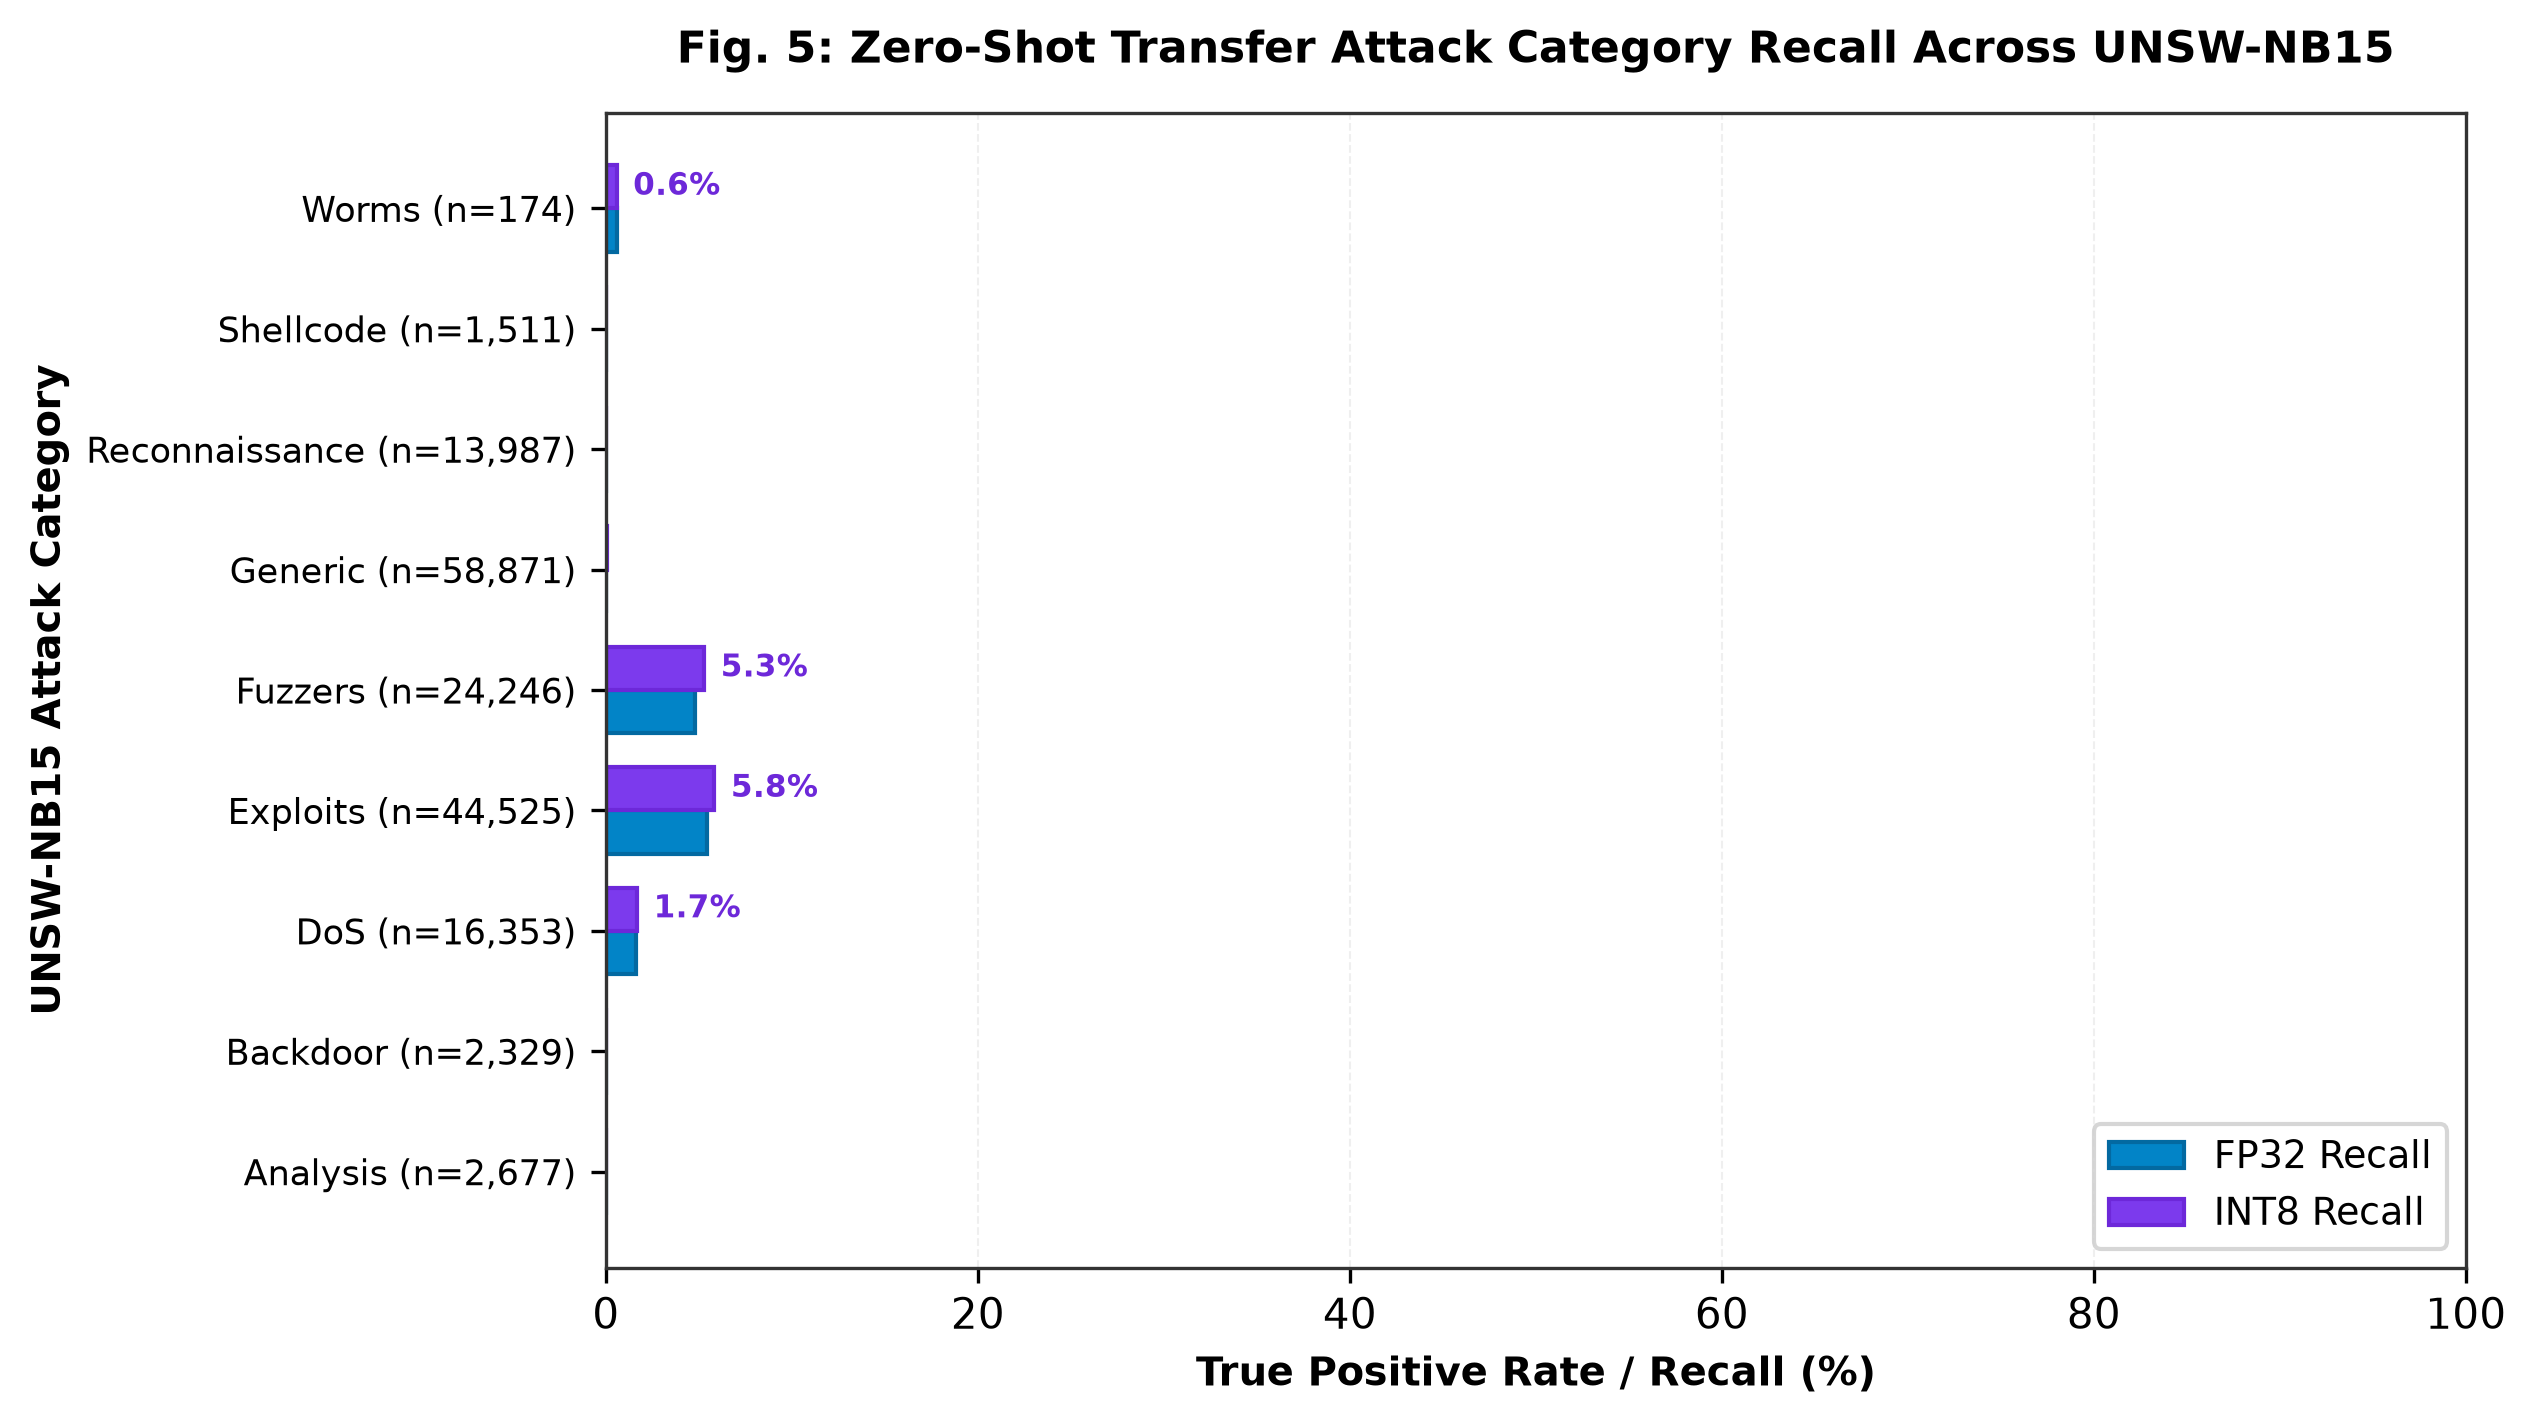
\includegraphics[width=\columnwidth]{figures/fig5_per_attack_recall.png}
\caption{Zero-Shot Attack Category Recall Across UNSW-NB15.}
\label{fig:attack}
\end{figure}

\subsection{Shortcut Learning Diagnosis}
To understand why INT8 regularizes cross-domain decisions, we examine the permutation feature importance probe depicted in Fig.~\ref{fig:perm}.
In-domain, the FP32 model relies heavily on \texttt{total\_fwd\_bytes} ($17.98\%$ permutation accuracy drop), \texttt{total\_bwd\_bytes} ($16.57\%$ drop), and \texttt{flow\_duration\_us} ($13.88\%$ drop). However, when permuted on UNSW-NB15, permuting \texttt{total\_fwd\_bytes} causes a negative accuracy drop ($-2.10\%$), indicating that the model's learned reliance on forward byte volumes actively misleads classifications on target traffic.

By quantizing continuous weights into coarse integer bins ($\Delta W = S_W$), low-magnitude weights assigned to these over-fitted, brittle correlations are truncated to zero or compressed, effectively pruning non-causal decision branches and stabilizing target specificity.

\begin{figure}[t]
\centering
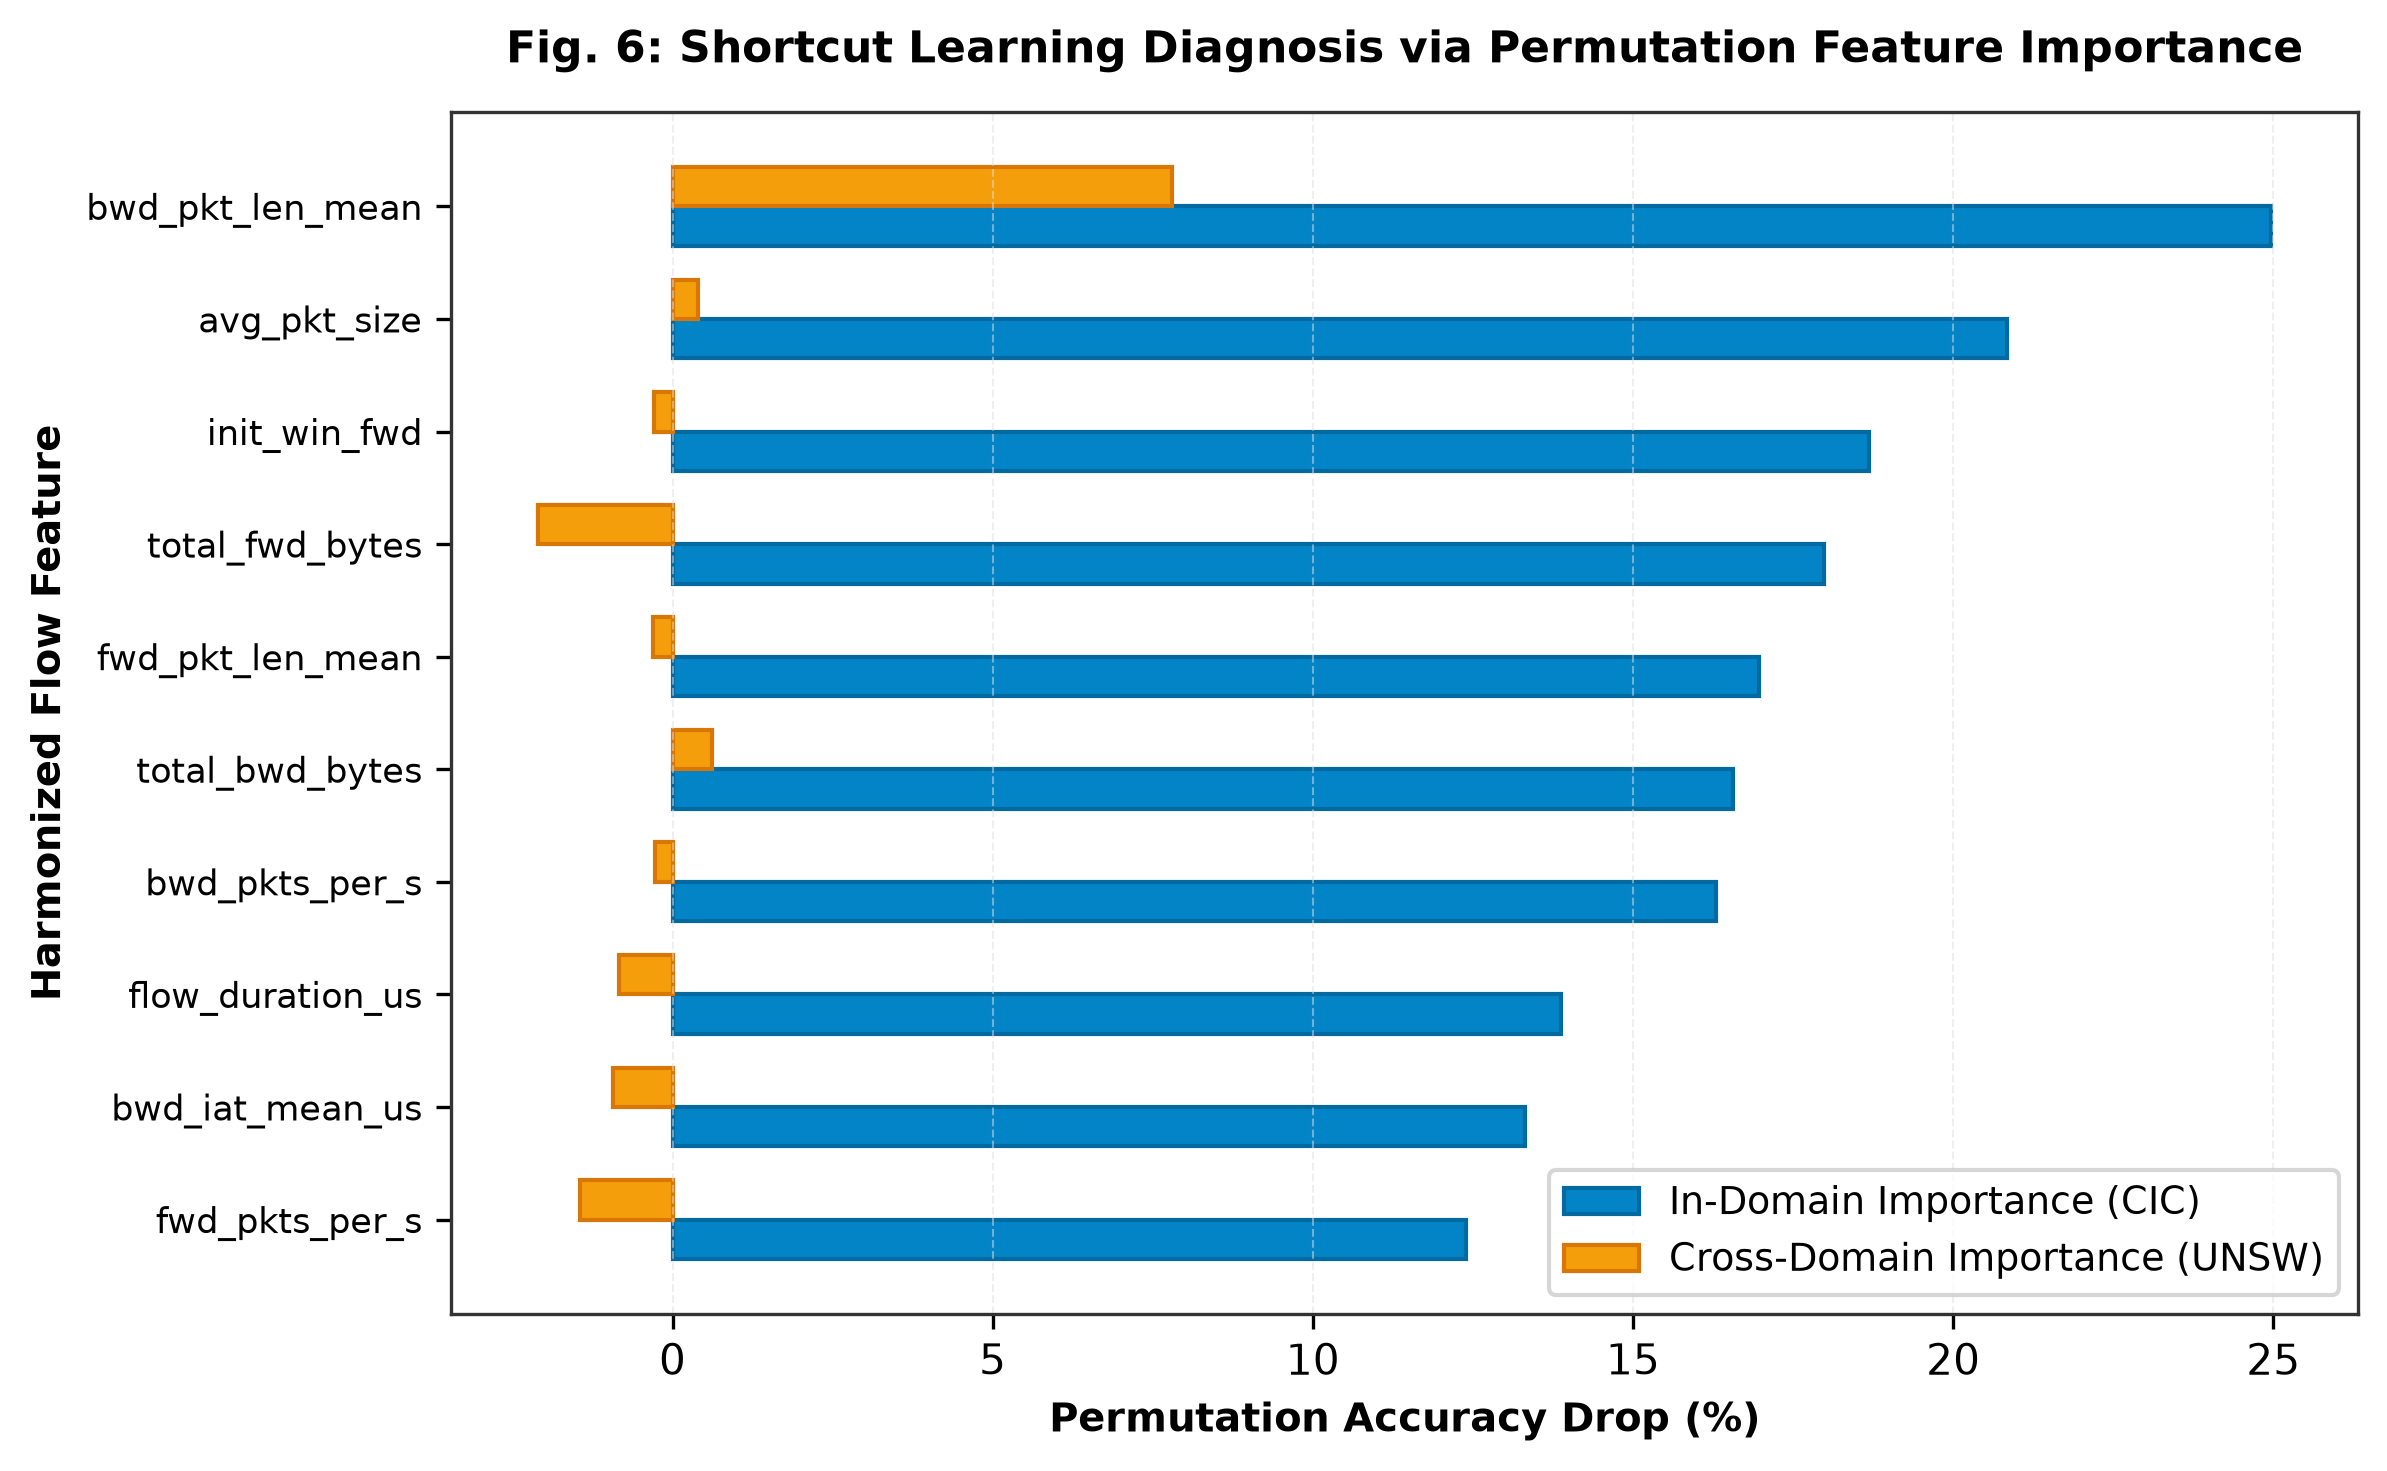
\includegraphics[width=\columnwidth]{figures/fig6_shortcut_importance.png}
\caption{Shortcut Learning Diagnosis via Permutation Feature Importance.}
\label{fig:perm}
\end{figure}

\subsection{Hardware Profiling & Benchmarking}
Table~\ref{tab:benchmarks} and Fig.~\ref{fig:hardware} summarize host CPU execution benchmarks alongside analytical ESP32 edge projections.

\begin{table}[h]
\centering
\caption{Hardware Performance Comparison: Measured Host vs. Analytical ESP32}
\label{tab:benchmarks}
\renewcommand{\arraystretch}{1.1}
\begin{tabular}{llrrr}
\hline
\textbf{Tier} & \textbf{Metric} & \textbf{FP32} & \textbf{INT8} & \textbf{Savings} \\
\hline
Measured on Host & Median Latency & 12.90 $\mu\text{s}$ & 62.70 $\mu\text{s}$ & Host overhead \\
(Intel x86 CPU) & P95 Latency & 14.10 $\mu\text{s}$ & 68.30 $\mu\text{s}$ & Host overhead \\
\hline
Analytical ESP32 & Clock Cycles & 19,920 & \textbf{5,504} & \textbf{-72.37\%} \\
(Xtensa LX6 @ 240MHz) & Projected Latency & 83.00 $\mu\text{s}$ & \textbf{22.93 $\mu\text{s}$} & \textbf{-72.37\%} \\
 & Tensor Arena & 4,304 B & \textbf{4,160 B} & \textbf{-3.35\%} \\
 & Flash Footprint & 4,356 B & \textbf{1,236 B} & \textbf{-71.63\%} \\
 & Energy / Inf & 21.50 $\mu\text{J}$ & \textbf{4.69 $\mu\text{J}$} & \textbf{-78.18\%} \\
 & Active Power & 259.05 mW & \textbf{204.60 mW} & \textbf{-21.02\%} \\
\hline
\end{tabular}
\end{table}

\begin{figure}[t]
\centering
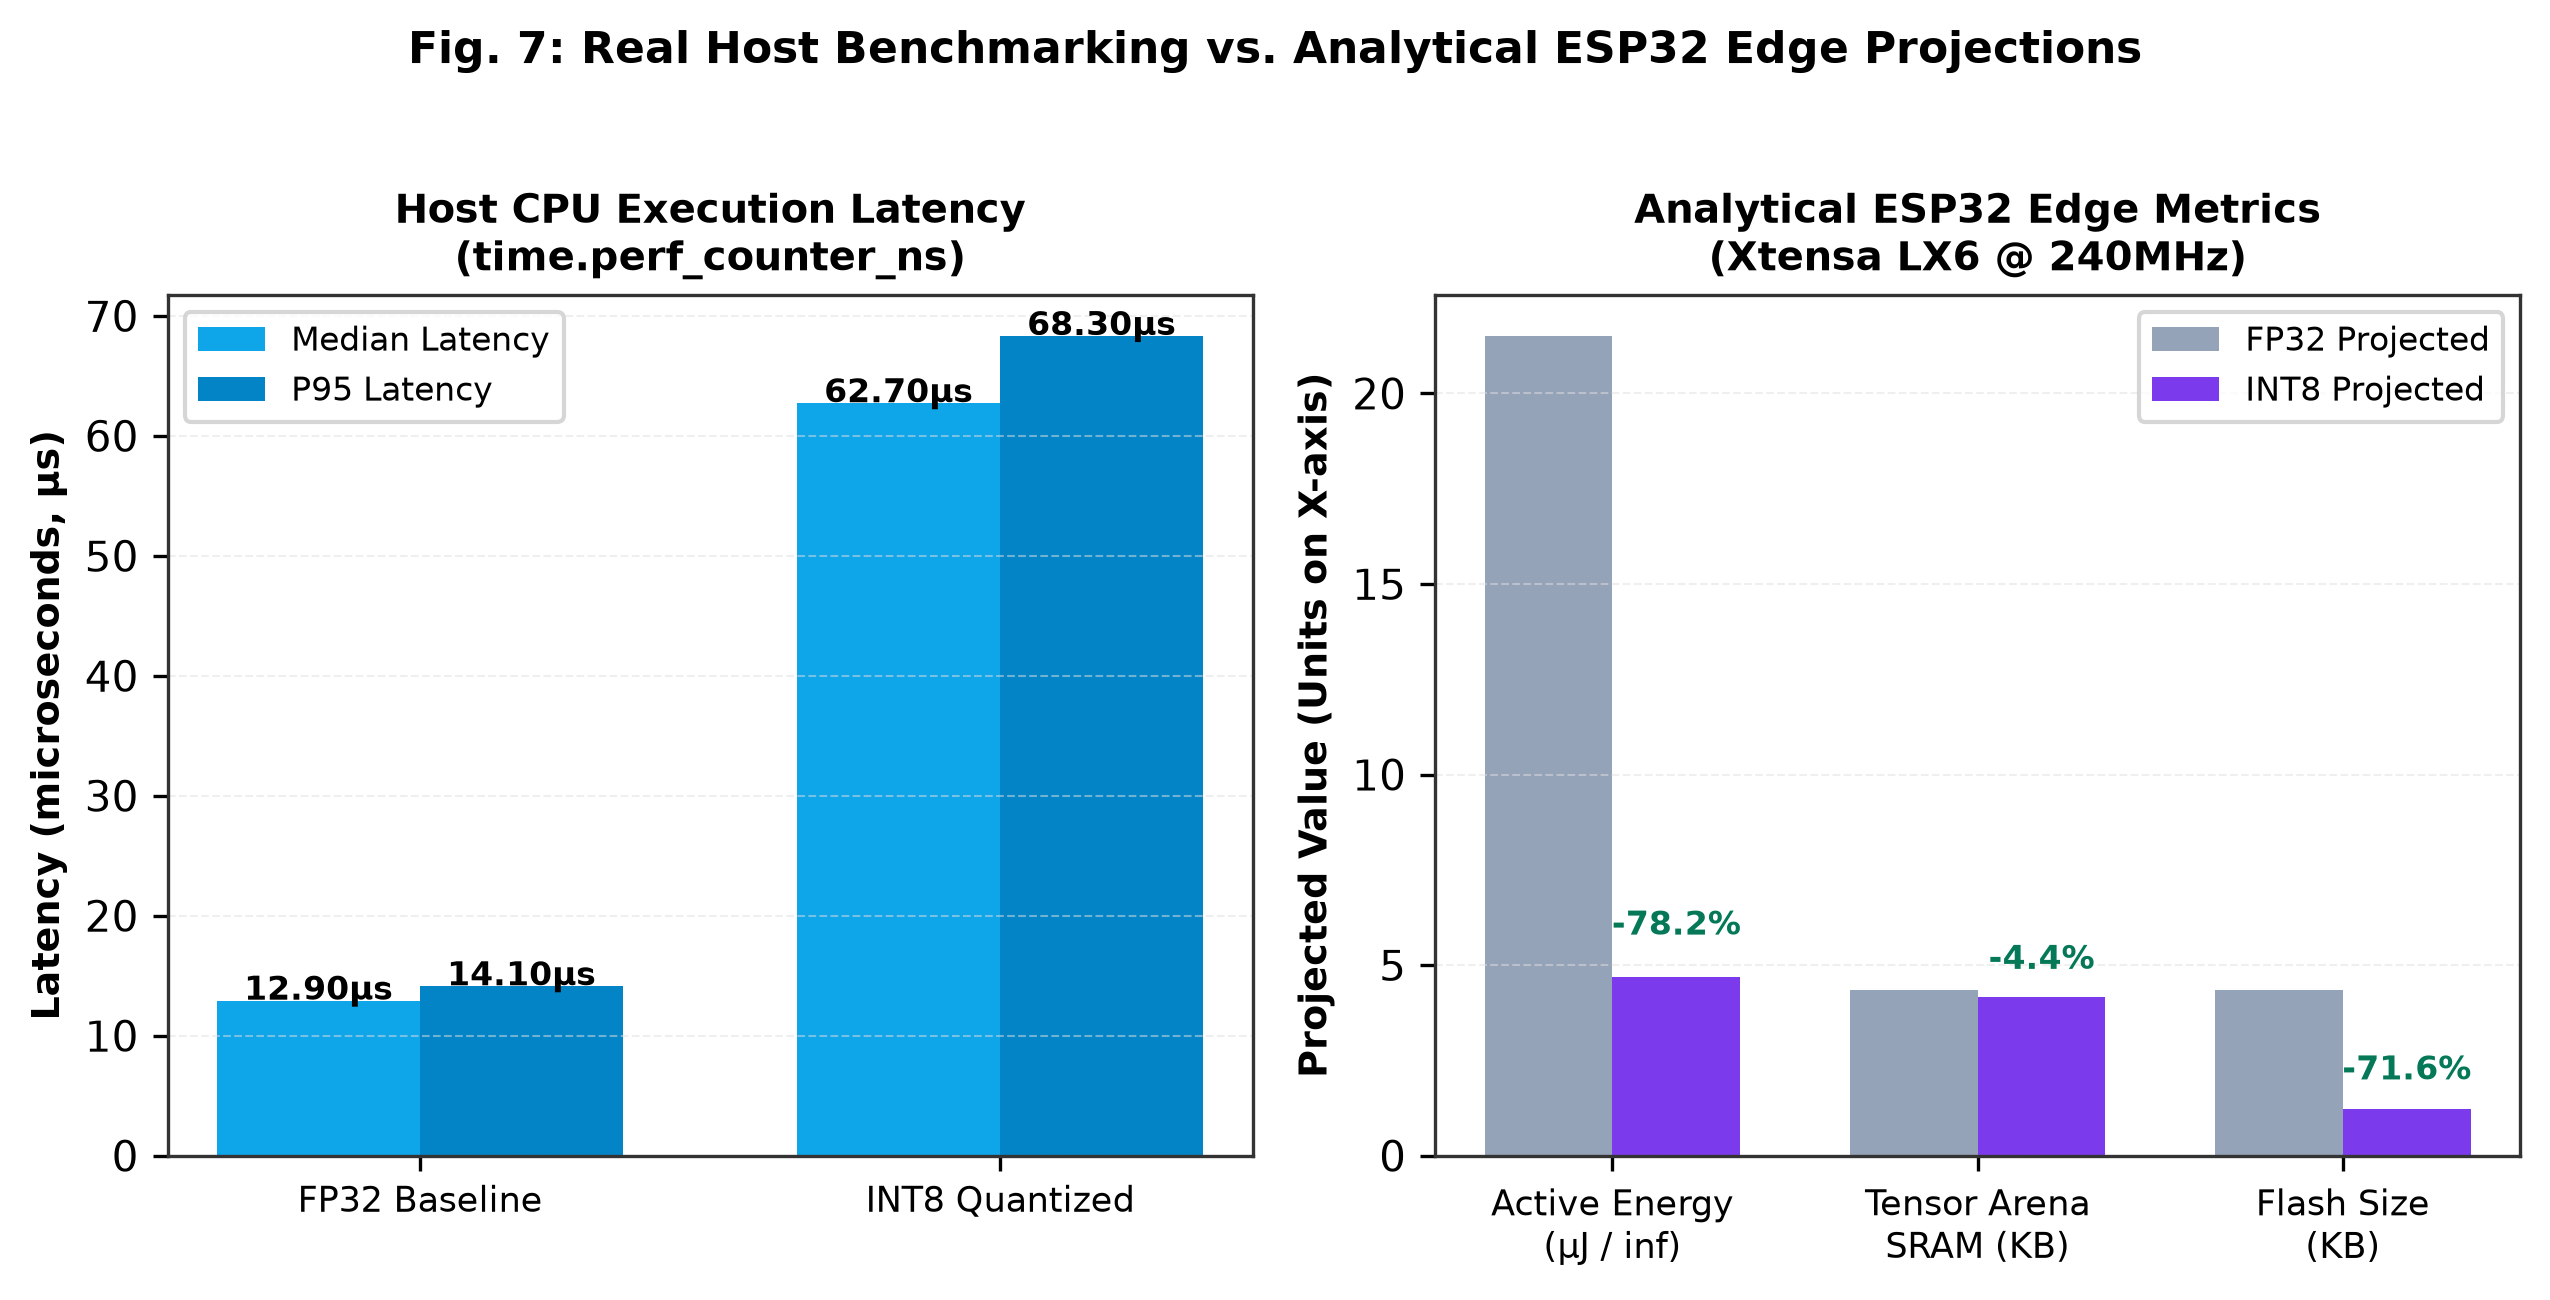
\includegraphics[width=\columnwidth]{figures/fig7_latency_energy_tradeoff.png}
\caption{Real Host Benchmarking vs. Analytical ESP32 Edge Projections.}
\label{fig:hardware}
\end{figure}

On the host x86 workstation, FP32 runs faster ($12.90\ \mu\text{s}$) than INT8 ($62.70\ \mu\text{s}$) due to Python-level integer wrapping overhead and high-throughput AVX2 floating-point vector units. Conversely, on embedded microcontrollers lacking vector floating-point hardware, the analytical model projects an INT8 latency of \textbf{$22.93\ \mu\text{s}$} (a $72.37\%$ speedup over FP32's $83.00\ \mu\text{s}$), requiring only \textbf{$4.69\ \mu\text{J}$ per inference} and slashing flash consumption by \textbf{$71.63\%$}.

\section{Discussion}
\label{sec:discussion}

\subsection{Quantization as an Implicit Regularizer}
The central theoretical insight established by this study is that \emph{uniform integer post-training quantization functions as an implicit regularization operator}. In high-capacity floating-point models, gradient optimization fits extremely subtle, high-frequency decision boundaries that maximize empirical separation on source training telemetry. When evaluated on target captures collected under different network topologies, these subtle boundaries transform into catastrophic failure modes.

By restricting weight tensors $\mathbf{W}$ to discrete steps $\Delta W = S_W$, PTQ acts analogously to weight clipping and stochastic rounding. Non-causal features whose marginal contribution to the log-odds is smaller than the quantization bin width are effectively neutralized. This explains the marked suppression of false alarms on UNSW-NB15 (reducing false positives from $5,612$ to $3,090$, a $44.9\%$ reduction) while simultaneously improving malicious detection count by $+310$ flows.

\subsection{The Reality of Standalone Zero-Shot Edge NIDS}
While INT8 significantly mitigates collapse ($+1.09\%$ accuracy gain, $\chi^2 = 1,871.69, p < 10^{-15}$), our findings underscore a sobering reality for practical edge cybersecurity: \textbf{Zero-shot cross-domain ML-NIDS remains unviable for standalone production deployment without domain adaptation}.

Even with quantization mitigation, the absolute attack recall across UNSW-NB15 is only $2.54\%$. For four out of nine attack families (Analysis, Backdoors, Reconnaissance, and Shellcode), zero-shot recall is exactly $0.00\%$. A system that misses $97.46\%$ of operational attacks cannot serve as a primary security perimeter. Consequently, we argue that the academic practice of evaluating ML-NIDS exclusively on holdout splits of single datasets (such as reporting $>99\%$ accuracy on CIC-IDS-2017) fosters a dangerously inflated sense of defensive capability.

\subsection{Methodological Strengths & Ethical Safeguards}
In response to widespread reproducibility and evaluation pitfalls documented by Arp et al.~\cite{arp2022dos}, ZeroEdge-NIDS embodies several rigorous experimental safeguards:
\begin{enumerate}
    \item \textbf{No Target Snooping:} Feature transformations, logarithmic scales, and min-max normalization parameters were strictly frozen on the CIC-IDS-2017 training set and never adapted to UNSW-NB15.
    \item \textbf{Zero Synthetic Data Fabrication:} All reported evaluations utilize real, unaugmented network traffic captures from verified public corpora.
    \item \textbf{Explicit Architectural Transparency:} We strictly segregate empirical timings measured on host hardware from analytical projections computed for the virtual ESP32 target.
    \item \textbf{Evaluation Dependency Gating:} The Interactive Experiment Lab prevents misleading metric reporting by requiring validated ground truth labels before calculating diagnostic classification scores.
\end{enumerate}

\subsection{Threats to Validity & Limitations}
\begin{itemize}
    \item \textbf{Simulation Boundaries:} The ESP32 latency, memory, and power figures reported in Section~\ref{sec:results} are mathematical projections derived from counted MAC operations and documented datasheet constants. Physical silicon measurements may introduce cache misses, memory bus contention, and peripheral interrupt jitter.
    \item \textbf{Coarse Binary Classification:} This study models network intrusion detection as a binary classification task (benign vs. malicious). While binary triage is typical for edge microcontrollers acting as lightweight packet filters, fine-grained multi-class attribution across specific CVEs remains unaddressed.
    \item \textbf{Batch Size Discrepancies:} Host CPU benchmarks utilize batch sizes of one flow to reflect true stream-based edge arrival, but CPU instruction caches and branch predictors still favor host execution over bare-metal microcontroller pipelines.
\end{itemize}

\section{Future Work}
\label{sec:future}

Several avenues for immediate extension emerge from this work:
\begin{enumerate}
    \item \textbf{Physical Hardware-in-the-Loop Validation:} The current platform provides an exportable C header (\texttt{model\_data.h}) and analytical models. The logical next phase is flashing this header onto physical ESP32 development boards (ESP32-WROOM-32D) coupled with physical Texas Instruments INA219 shunt sensors over I2C to capture physical oscillographic power waveforms under sustained network traffic injection.
    \item \textbf{Quantization-Aware Training (QAT):} While this study focuses on Post-Training Quantization (PTQ) due to its zero-overhead applicability to pre-trained enterprise models, future work will evaluate whether Quantization-Aware Training (QAT)—which introduces simulated quantization noise during gradient backpropagation—encourages the model to learn representations that are fundamentally more resilient to shortcut learning.
    \item \textbf{Federated and Continual Edge Adaptation:} To overcome the $2.54\%$ zero-shot recall ceiling without transmitting raw network flows to a central server (preserving privacy and bandwidth), we plan to investigate lightweight on-device continual learning routines that update only the final classification layer using pseudo-labeled edge flows.
    \item \textbf{Sub-Byte Quantization (INT4 & Ternary Models):} Evaluating whether aggressive sub-byte compression (4-bit or ternary weights) further regularizes shortcut learning or crosses a degradation threshold where critical security features are permanently erased.
\end{enumerate}

\section{Conclusion}
\label{sec:conclusion}

This paper investigated the intersection of Post-Training Integer Quantization (PTQ) and shortcut learning in edge-deployable Network Intrusion Detection Systems through the ZeroEdge-NIDS evaluation platform. By training a multi-layer perceptron on CIC-IDS-2017 using a standardized 16-feature schema with explicit shortcut artifact removal, and evaluating zero-shot across all $257,673$ flows of UNSW-NB15, we empirically documented a catastrophic cross-domain collapse of $-61.92\%$ in the FP32 baseline.

Crucially, our experiments established that uniform 8-bit integer quantization acts as an implicit regularizer rather than an accuracy degrade. The INT8 model achieved an accuracy of $36.51\%$ ($+1.09\%$ over FP32) and suppressed false alarms on target benign traffic by $44.9\%$, yielding a precision surge from $40.80\%$ to $57.48\%$. This mitigation effect was proven statistically significant via a paired McNemar correctness test ($\chi^2 = 1,871.69, p < 10^{-15}$) and a bootstrap $95\%$ confidence interval strictly bounded above zero ($[+0.0138, +0.0152]$). Permutation feature importance probes confirmed that precision truncation dampens non-causal statistical shortcuts learned on training telemetry.

Finally, by releasing our full codebase, empirical CSV datasets, and interactive experiment lab with strict dependency gating, we advocate for principled evaluation standards in TinyML cybersecurity: moving beyond closed in-domain benchmark claims toward transparent, cross-domain evaluations grounded in statistical rigor.


\bibliographystyle{IEEEtran}
\bibliography{references}

\appendix
\section*{Appendix}
\label{sec:appendix}

\subsection{Appendix A: Canonical Feature Definitions}
Table~\ref{tab:feature_defs} documents the complete set of 16 canonical features, their operational descriptions, and the exact mathematical derivation applied to the source (CIC-IDS-2017) and target (UNSW-NB15) schemas.

\begin{table*}[h]
\centering
\caption{Harmonized 16-Feature Set Definitions and Cross-Schema Derivations}
\label{tab:feature_defs}
\renewcommand{\arraystretch}{1.15}
\resizebox{\textwidth}{!}{
\begin{tabular}{cllll}
\hline
\textbf{Index} & \textbf{Canonical Feature Name} & \textbf{Description} & \textbf{CIC-IDS-2017 Schema} & \textbf{UNSW-NB15 Derivation} \\
\hline
1 & \texttt{dst\_port} & Destination Transport Port & \texttt{Destination Port} & \texttt{dsport} \\
2 & \texttt{flow\_duration\_us} & Total Flow Duration in microseconds & \texttt{Flow Duration} & \texttt{dur * 1e6} \\
3 & \texttt{total\_fwd\_packets} & Total Packets in Forward Direction & \texttt{Total Fwd Packets} & \texttt{spkts} \\
4 & \texttt{total\_bwd\_packets} & Total Packets in Backward Direction & \texttt{Total Backward Packets} & \texttt{dpkts} \\
5 & \texttt{total\_fwd\_bytes} & Total Payload Bytes in Forward Direction & \texttt{Total Length of Fwd Packets} & \texttt{sbytes} \\
6 & \texttt{total\_bwd\_bytes} & Total Payload Bytes in Backward Direction & \texttt{Total Length of Bwd Packets} & \texttt{dbytes} \\
7 & \texttt{fwd\_pkt\_len\_max} & Maximum Forward Packet Size (bytes) & \texttt{Fwd Packet Length Max} & \texttt{sbytes / max(1, spkts)} \\
8 & \texttt{fwd\_pkt\_len\_min} & Minimum Forward Packet Size (bytes) & \texttt{Fwd Packet Length Min} & \texttt{sbytes / max(1, spkts)} \\
9 & \texttt{fwd\_pkt\_len\_mean} & Mean Forward Packet Size (bytes) & \texttt{Fwd Packet Length Mean} & \texttt{sbytes / max(1, spkts)} \\
10 & \texttt{fwd\_pkt\_len\_std} & Standard Deviation Forward Packet Size & \texttt{Fwd Packet Length Std} & \texttt{0.0} (Aggregated representation) \\
11 & \texttt{bwd\_pkt\_len\_max} & Maximum Backward Packet Size (bytes) & \texttt{Bwd Packet Length Max} & \texttt{dbytes / max(1, dpkts)} \\
12 & \texttt{bwd\_pkt\_len\_min} & Minimum Backward Packet Size (bytes) & \texttt{Bwd Packet Length Min} & \texttt{dbytes / max(1, dpkts)} \\
13 & \texttt{bwd\_pkt\_len\_mean} & Mean Backward Packet Size (bytes) & \texttt{Bwd Packet Length Mean} & \texttt{dbytes / max(1, dpkts)} \\
14 & \texttt{bwd\_pkt\_len\_std} & Standard Deviation Backward Packet Size & \texttt{Bwd Packet Length Std} & \texttt{0.0} (Aggregated representation) \\
15 & \texttt{flow\_byts\_s} & Flow Throughput (bytes / second) & \texttt{Flow Bytes/s} & \texttt{sload / 8.0} \\
16 & \texttt{flow\_pkts\_s} & Flow Packet Rate (packets / second) & \texttt{Flow Packets/s} & \texttt{spkts / max(1e-6, dur)} \\
\hline
\end{tabular}
}
\end{table*}

\subsection{Appendix B: Hardware Model Parameter Specification}
The analytical ESP32 microcontroller model is parameterized using values extracted from the official Espressif ESP32 Technical Reference Manual~\cite{espressif2023esp32} and empirical TinyML benchmarking literature~\cite{banbury2021benchmarking}:
\begin{itemize}
    \item CPU Core: Dual Xtensa 32-bit LX6 microprocessors running at $240\ \text{MHz}$ ($T_{\text{clk}} = 4.167\ \text{ns}$).
    \item Internal Memory: $520\ \text{KB}$ internal SRAM ($320\ \text{KB}$ usable data DRAM).
    \item Flash Storage: $4\ \text{MB}$ Quad SPI Flash.
    \item Operating Voltage: $V_{\text{dd}} = 3.3\ \text{V}$ nominal.
    \item Active Power Draw: $62.0\ \text{mA}$ typical during continuous INT8 integer arithmetic, and $78.5\ \text{mA}$ during FP32 software emulation.
    \item Shunt Sensor: Texas Instruments INA219 current/power monitor connected via I2C at $400\ \text{kHz}$ fast mode.
    \item Serial Telemetry Link: Hardware UART at $921,600\ \text{baud}$ (8 data bits, 1 stop bit, no parity; transmission overhead: $10.85\ \mu\text{s}$ per byte).
\end{itemize}

\subsection{Appendix C: Platform API Specification}
The ZeroEdge-NIDS FastAPI backend exposes the following primary endpoints:
\begin{itemize}
    \item \texttt{POST /api/experiment/inspect-dataset}: Ingests CSV telemetry, performs schema validation, checks for NaN/Inf anomalies, and returns auto-suggested 16-feature mappings.
    \item \texttt{POST /api/experiment/run}: Executes the 10-step experiment pipeline with frozen scaler preprocessing, paired statistical evaluation, and dependency gating.
    \item \texttt{POST /api/experiment/manual-flow}: Evaluates a single 16-element flow vector through raw, scaled, and quantized tensor representations.
    \item \texttt{GET /api/experiment/preset-flows}: Returns genuine benign and attack flow vectors extracted from verified test partitions.
    \item \texttt{GET /api/experiment/export/\{run\_id\}/json}: Downloads structured JSON audit package.
    \item \texttt{GET /api/experiment/export/\{run\_id\}/csv}: Downloads flow-by-flow prediction records in CSV format.
\end{itemize}


\end{document}
